% =========================================================
% MODELO ABNT - RELATÓRIO TÉCNICO DE SOFTWARE (RTS)
% Instituto Federal do Piauí – Curso Superior de ADS
% Autor - Prof Ricardo Moura Sekeff Budaruiche
% =========================================================

\documentclass[12pt,openright,oneside,a4paper]{article}

% ---------------------------------------------------------
% PACOTES BÁSICOS
\usepackage[T1]{fontenc}
\usepackage[utf8]{inputenc}
\usepackage[brazil]{babel}
\usepackage{times}
\usepackage{setspace}
\usepackage{geometry}
\usepackage{graphicx}
\usepackage{float}
\usepackage{listings}
\usepackage{xcolor}
\usepackage{caption}
\usepackage{booktabs}
\usepackage{hyperref}
\usepackage{amsmath, amssymb}
\usepackage{indentfirst}
\usepackage{lipsum}
\usepackage{enumerate}

\lstset{
    language=Python,            % linguagem padrão (pode trocar)
    basicstyle=\ttfamily\small, % fonte do código
    emph={@app},              % palavras que queremos colorir
    emphstyle=\color{teal}\bfseries,        % estilo delas
    keywordstyle=\color{blue}\bfseries,  % cor das palavras-chave
    backgroundcolor=\color{black!5},
    stringstyle=\color{red},
    commentstyle=\color{gray},
    showstringspaces=false,
    breaklines=true,
    frame=single,               % coloca borda
    numbers=left,               % numeração de linhas
    numberstyle=\tiny\color{gray},
    tabsize=4
}

% Define a linguagem JavaScript/TypeScript para o listings (não é embutida).
% Sem isto, \begin{lstlisting}[language=JavaScript] falha ao carregar a linguagem
% e deixa a fonte monoespaçada (\ttfamily) ativa no restante do documento.
\lstdefinelanguage{JavaScript}{
    morekeywords={await, async, function, return, const, let, var, if, else,
        for, while, throw, new, try, catch, finally, export, import, from,
        default, typeof, true, false, null, undefined, class, extends},
    sensitive=true,
    comment=[l]{//},
    morecomment=[s]{/*}{*/},
    morestring=[b]",
    morestring=[b]',
    morestring=[b]`
}

\renewcommand{\lstlistingname}{Código}
\renewcommand{\lstlistlistingname}{Lista de Códigos}
% ---------------------------------------------------------
% FORMATAÇÃO
% ---------------------------------------------------------
\geometry{a4paper, left=3cm, right=2cm, top=2.5cm, bottom=2.5cm}
\setstretch{1.5}
\captionsetup{labelfont=bf, labelsep=endash}

% ---------------------------------------------------------
% DADOS DO TRABALHO
% ---------------------------------------------------------
\newcommand{\Instituicao}{INSTITUTO FEDERAL DE EDUCAÇÃO, CIÊNCIA E TECNOLOGIA DO PIAUÍ}
\newcommand{\Campus}{Campus Piripiri}
\newcommand{\Curso}{Tecnólogo em Análise e Desenvolvimento de Sistemas}
\newcommand{\Titulo}{MOVY: PLATAFORMA SAAS PARA GERENCIAMENTO DE TRANSPORTE UNIVERSITÁRIO INTERMUNICIPAL COM ARQUITETURA MULTITENANCY}
\newcommand{\Autor}{Rauan dos Santos Bandeira}
\newcommand{\Orientador}{Jeferson Soares}
\newcommand{\CoOrientador}{Nome do(a) Coorientador(a) (opcional)}
\newcommand{\Cidade}{Piripiri – PI}
\newcommand{\Ano}{2026}

% ---------------------------------------------------------
\begin{document}

% ================= CAPA =====================
\begin{titlepage}
\begin{center}
\includegraphics[width=10cm]{imagens/Logo-IFPI-Vertical.png} \\[0.3cm]
\textbf{\Instituicao} \\
\textbf{\Campus} \\
\textbf{\Curso} \\[3cm]

\textbf{\Autor} \\[2.5cm]
\textbf{\Titulo} \\[6cm]

\Cidade\\
\Ano
\end{center}
\end{titlepage}

% ================= FOLHA DE ROSTO =====================
\begin{titlepage}
\begin{center}
\textbf{\Autor} \\[3cm]

\textbf{\Titulo} \\[2cm]

\begin{flushright}
Relatório Técnico de Software apresentado ao curso de \Curso{}, como requisito parcial para a conclusão do Trabalho de Conclusão de Curso (TCC). \\
Orientador(a): \Orientador \\
Coorientador(a): \CoOrientador
\end{flushright}

\vfill
\Cidade \\
\Ano
\end{center}
\end{titlepage}

% ================= RESUMO =====================
\newpage
\section*{Resumo}

A organização do transporte universitário intermunicipal ainda ocorre, em muitas localidades, de forma manual e pouco estruturada — com listas informais em aplicativos de mensagens, ausência de controle de capacidade e gestão financeira frágil. Este trabalho apresenta o \textbf{Movy}, uma plataforma de \textit{Software as a Service} (SaaS) concebida para automatizar o agendamento de viagens, o registro de passageiros e o controle financeiro desse serviço. O sistema é composto por dois artefatos integrados: uma \textbf{API REST} escalável, responsável pela lógica de domínio e pela persistência, e uma \textbf{aplicação web cliente} \textit{mobile-first}, responsável por toda a interação com o usuário. A API foi desenvolvida em NestJS com TypeScript, Prisma ORM e PostgreSQL, segundo os princípios de \textit{Clean Architecture} e \textit{Domain-Driven Design} (DDD), implementando arquitetura \textit{multi-tenant} com isolamento lógico de dados por organização, autenticação JWT, controle de acesso baseado em papéis (RBAC), transações atômicas e limites de plano. O cliente, em React e TanStack Router, espelha a separação em camadas do servidor e materializa, em telas e fluxos, os requisitos expostos pela API, delegando a ela toda decisão de negócio. Foram implementados os treze módulos funcionais previstos — totalizando 93 \textit{endpoints} REST — e a verificação do backend conta com 458 testes unitários em 57 \textit{suites}. Os resultados indicam que a arquitetura adotada oferece uma base sólida, segura e manutenível para a operação do serviço, com pontos de evolução claramente identificados.

\textbf{Palavras-chave:} Transporte universitário; SaaS; API REST; Multi-tenancy; NestJS; React; DDD; Clean Architecture.

\newpage
\section*{Abstract}

In many locations, the organization of intercity university transportation is still carried out manually and in an unstructured way — relying on informal lists in messaging apps, with no capacity control and weak financial management. This work presents \textbf{Movy}, a \textit{Software as a Service} (SaaS) platform designed to automate trip scheduling, passenger registration, and financial control of this service. The system comprises two integrated artifacts: a scalable \textbf{REST API}, responsible for domain logic and persistence, and a \textit{mobile-first} \textbf{web client application}, responsible for all user interaction. The API was developed in NestJS with TypeScript, Prisma ORM, and PostgreSQL, following \textit{Clean Architecture} and \textit{Domain-Driven Design} (DDD) principles, implementing a \textit{multi-tenant} architecture with logical data isolation per organization, JWT authentication, role-based access control (RBAC), atomic transactions, and plan limits. The client, built with React and TanStack Router, mirrors the server's layered separation and materializes, in screens and flows, the requirements exposed by the API, delegating all business decisions to it. The thirteen planned functional modules were implemented — totaling 93 REST endpoints — and backend verification comprises 458 unit tests across 57 suites. The results indicate that the adopted architecture provides a solid, secure, and maintainable foundation for operating the service, with clearly identified evolution points.

\textbf{Keywords:} University transportation; SaaS; REST API; Multi-tenancy; NestJS; React; DDD; Clean Architecture.

% ================= SUMÁRIO =====================
\newpage
\tableofcontents
% \lstlistoflistings % Para exibir a lista de listagens de códigos
\newpage

% ================= DESENVOLVIMENTO =====================
\section{Introdução}
\label{sec:introducao}
O ensino superior presencial no Brasil apresenta uma expressiva dimensão e mantém milhões de estudantes matriculados ao longo dos últimos anos. Dados do Censo da Educação Superior, divulgados pelo Instituto Nacional de Estudos e Pesquisas Educacionais Anísio Teixeira (INEP), indicam que, em 2010, o país registrava 5.476.813 matrículas presenciais, número que se manteve elevado, alcançando 5.037.875 matrículas em 2024, distribuídas em 2.444 instituições de ensino superior presenciais \cite{inepCensoSuperior}. Esses dados evidenciam que uma parcela significativa dos universitários depende da frequência física às instituições para a realização de suas atividades acadêmicas.

Essa realidade é reforçada por informações do Censo Demográfico de 2022, realizado pelo Instituto Brasileiro de Geografia e Estatística (IBGE), que apontam que 27,3\% dos estudantes de graduação cursam o ensino superior em município diferente daquele em que residem \cite{ibgeDeslocamentoEstudo}. Esse cenário evidencia que o deslocamento intermunicipal faz parte da rotina de uma parcela significativa dos universitários, especialmente em regiões onde a oferta de cursos presenciais está concentrada em cidades-polo.

Apesar da importância do transporte universitário intermunicipal para a permanência desses estudantes no ensino superior, a organização desse serviço ainda ocorre, em muitas localidades, de forma manual e pouco estruturada. O agendamento das viagens e o controle de presença são frequentemente realizados por meio de listas informais em aplicativos de mensagens, como grupos de WhatsApp, nos quais os alunos registram seus nomes para confirmar a participação. Esse modelo de gestão está sujeito a falhas, como duplicidade de registros, esquecimentos, dificuldades de comunicação e ausência de controle financeiro adequado.

O cenário foi observado diretamente na prática, durante a utilização diária do serviço em uma rota específica.  Constatou-se que a inexistência de um sistema informatizado compromete a visualização clara dos passageiros confirmados, dificulta o gerenciamento dos pagamentos e aumenta o risco de decisões equivocadas quanto à viabilidade das viagens, uma vez que, em muitos casos, há um número mínimo de passageiros necessário para que o deslocamento ocorra. Dessa forma, problemas como atrasos, prejuízos financeiros e desorganização tornam-se recorrentes.

Diante desse contexto, evidencia-se a necessidade de uma solução tecnológica capaz de automatizar o processo de agendamento de viagens, o registro de passageiros e o controle financeiro do transporte universitário intermunicipal, proporcionando maior organização, confiabilidade e eficiência tanto para os estudantes quanto para os responsáveis pelo serviço.

Para responder a essa necessidade, este trabalho apresenta o \textbf{Movy}, sistema concebido como dois artefatos integrados e complementares: uma \textbf{API REST} (\textit{backend}), que concentra as regras de negócio e a persistência, e uma \textbf{aplicação web cliente} (\textit{frontend}) \textit{mobile-first}, que materializa essas regras em telas e fluxos para os perfis de passageiro, motorista e administrador. Um princípio condutor de todo o projeto é que o cliente \textbf{não detém regras de negócio autoritativas}: ele orquestra a interação e valida entradas localmente apenas para fornecer retorno imediato, delegando toda decisão definitiva à API. Por essa razão, este relatório descreve o sistema de forma unificada, tratando \textit{backend} e \textit{frontend} como duas camadas de um mesmo produto sempre que o tema é comum (requisitos, modelo de domínio, arquitetura, segurança), e os diferenciando apenas quando a implementação assim exige.

\subsection{Objetivos}

\subsubsection{Objetivo Geral}
Desenvolver o sistema Movy --- composto por uma API REST escalável e por uma aplicação web cliente que a consome --- para o gerenciamento do transporte universitário intermunicipal, automatizando o agendamento de viagens, o registro de passageiros e o controle financeiro, de modo a proporcionar maior organização, transparência e eficiência para estudantes e responsáveis pelo transporte.

\subsubsection{Objetivos Específicos}
\begin{itemize}
\item Analisar o funcionamento atual do transporte universitário intermunicipal, identificando problemas e limitações dos processos manuais adotados;
\item Levantar e documentar os requisitos funcionais e não funcionais do sistema, com base nas necessidades dos estudantes e dos responsáveis pelo transporte;
\item Projetar a arquitetura do sistema, definindo a separação em camadas do servidor e do cliente, os padrões de comunicação e a estrutura do banco de dados;
\item Modelar os principais artefatos do sistema, incluindo casos de uso, modelo de domínio e modelo entidade-relacionamento;
\item Implementar a API REST utilizando tecnologias adequadas ao desenvolvimento de sistemas \textit{back-end};
\item Implementar a aplicação cliente que consome a API, com controle de acesso por papel e comunicação resiliente;
\item Realizar testes funcionais e unitários para validar o correto funcionamento das principais funcionalidades implementadas;
\item Avaliar os resultados obtidos com a solução desenvolvida, considerando aspectos de organização, confiabilidade e facilidade de uso.
\end{itemize}


% ------------------------------
\section{Trabalhos Relacionados}

Diversos estudos têm abordado o uso de sistemas de informação no gerenciamento de transporte estudantil e universitário, com o objetivo de otimizar processos, reduzir falhas operacionais e melhorar a organização das viagens.

O trabalho PickBus, proposto por Pretto et al. \cite{pickbus2021}, apresenta uma solução multiplataforma (web e mobile) voltada ao gerenciamento de transporte fretado de passageiros, com foco em eventos e deslocamentos coletivos. O sistema permite a criação e o gerenciamento de viagens, controle de passageiros, organização de pagamentos e centralização da comunicação entre organizadores e usuários. O estudo fundamenta-se em conceitos de mobilidade urbana e empreendedorismo, demonstrando a viabilidade da solução por meio de pesquisa de mercado e testes com usuários reais. Os resultados indicam boa aceitação do sistema e evidenciam a carência de ferramentas digitais específicas para o gerenciamento de transporte fretado.


O trabalho intitulado "Sistema para Gerenciamento de Transportes", desenvolvido por Anderson et al. \cite{anderson2020}, apresenta uma solução voltada à modernização do processo de solicitação e gerenciamento de transportes no contexto de uma instituição acadêmica. A proposta surge da necessidade de substituir métodos manuais baseados em troca de e-mails, os quais são suscetíveis a falhas de comunicação e perda de informações. O sistema permite o cadastro e a gestão de veículos, motoristas e setores, bem como a solicitação de viagens, verificação de disponibilidade, fluxo de aprovação hierárquico e alocação de recursos. Além disso, a solução contempla funcionalidades de monitoramento por meio de painéis e geração de relatórios, contribuindo para maior transparência e apoio à tomada de decisão. O estudo evidencia que a informatização do processo de gestão de transportes institucionais promove maior organização, eficiência operacional e confiabilidade das informações.


Outro trabalho relevante é o de Reis et al. \cite{reis2021transporte}, que apresenta a modelagem de um software voltado ao gerenciamento do transporte escolar público municipal. A proposta tem como foco o levantamento de requisitos e a utilização de técnicas de Engenharia de Software e UML para organizar informações relacionadas a alunos, rotas, veículos, motoristas e monitores. O estudo evidencia que a ausência de sistemas informatizados compromete a eficiência operacional e a tomada de decisão, especialmente em contextos com grande volume de usuários e necessidade de relatórios precisos. Diferentemente do presente projeto, que se concentra no transporte universitário intermunicipal e na oferta de uma API escalável para integração com diferentes aplicações cliente, o trabalho de Reis et al. (2021) enfatiza a modelagem conceitual e o contexto do ensino básico municipal, reforçando, contudo, a importância da informatização como fator essencial para a organização e confiabilidade dos serviços de transporte educacional.

O sistema proposto neste trabalho diferencia-se das soluções analisadas por abordar de forma específica o contexto do transporte universitário intermunicipal, um cenário ainda pouco explorado na literatura, sobretudo no que se refere à integração entre organização operacional e controle financeiro. Enquanto os trabalhos relacionados concentram-se no transporte escolar, no fretamento eventual para eventos ou na gestão institucional de veículos, a presente proposta foca nas particularidades do deslocamento diário e recorrente de estudantes universitários entre municípios, considerando suas demandas operacionais e administrativas.

Além da automatização do agendamento de viagens, do gerenciamento da lista de passageiros e da centralização da comunicação entre usuários e responsáveis pelo transporte, o principal diferencial do sistema está na inclusão de um módulo de controle financeiro integrado à gestão das viagens. O sistema permite a estimativa automática da arrecadação por viagem com base no número de passageiros confirmados, possibilitando ao responsável avaliar rapidamente a viabilidade financeira de cada deslocamento.

Adicionalmente, ao ser concebido como uma API escalável com modelo SaaS multi-tenant, acompanhada de uma aplicação cliente própria, o projeto amplia sua aplicabilidade, permitindo a integração com diferentes sistemas clientes, como aplicações web ou móveis, o que não é observado nos trabalhos analisados.


% ------------------------------
\section{Tecnologias Implementadas}

A seleção tecnológica foi orientada pelos requisitos de escalabilidade, segurança e manutenibilidade no servidor, e por produtividade, segurança de tipos e caráter \textit{mobile-first} no cliente. As duas camadas compartilham a linguagem TypeScript, o que estabelece contratos de dados explícitos entre elas. As subseções a seguir apresentam, separadamente, a \textit{stack} de cada camada e a justificativa das principais escolhas.

\subsection{Stack do Backend}

A adoção de NestJS foi fundamentada na necessidade de uma arquitetura estruturada, com suporte nativo a padrões como injeção de dependência, módulos, \textit{guards} e interceptadores globais, essenciais para implementar \textit{Clean Architecture} e RBAC de forma consistente.

\begin{table}[H]
\centering
\caption{Tecnologias implementadas no backend (Movy API)}
\label{tab:tecnologias_implementadas}
\begin{tabular}{lll}
\toprule
\textbf{Tecnologia} & \textbf{Versão} & \textbf{Descrição} \\
\midrule
Node.js & v18+ & Ambiente de execução JavaScript/TypeScript \\
TypeScript & 5.3+ & Linguagem tipada para desenvolvimento seguro \\
NestJS & v11.0+ & Framework backend modular com DI nativo\\
Prisma ORM & v7.5+ & ORM com tipagem forte e migrations automáticas \\
PostgreSQL & 15+ & SGBD relacional para persistência de dados \\
JWT (NestJS/Passport) & 11.0+ & Implementação de autenticação com tokens \\
Bcrypt & 6.0+ & Hash seguro de senhas com salt rounds \\
Docker & Latest & Conteinerização e orquestração de ambientes \\
Jest & 30+ & Framework de testes unitários e de integração \\
ESLint & 9+ & Análise estática de código TypeScript \\
Swagger & 11.2+ & Documentação interativa de endpoints REST \\
@nestjs/schedule & 6.1+ & Agendamento de \textit{jobs} (cron) de viagens \\
@nestjs/throttler & 6.5+ & \textit{Rate limiting} global (60 req/min) \\
\bottomrule
\end{tabular}
\end{table}

\subsection{Stack do Frontend}

A seleção tecnológica do cliente priorizou produtividade de desenvolvimento, segurança de tipos --- alinhada ao \textit{backend} em TypeScript --- e adequação ao caráter \textit{mobile-first} do produto. A Tabela~\ref{tab:tecnologias_frontend} resume a \textit{stack} adotada.

\begin{table}[H]
\centering
\caption{Tecnologias implementadas no frontend (aplicação cliente)}
\label{tab:tecnologias_frontend}
\begin{tabular}{lll}
\toprule
\textbf{Tecnologia} & \textbf{Versão} & \textbf{Descrição} \\
\midrule
React & 19.2 & Biblioteca de interface declarativa baseada em componentes \\
TypeScript & 5.8 & Linguagem tipada; contratos explícitos com a API \\
TanStack Router & 1.16+ & Roteamento \textit{file-based} com segurança de tipos \\
TanStack Start & 1.16+ & Camada \textit{full-stack} (SSR opcional) sobre o Router \\
Tailwind CSS & 4.2 & Estilização \textit{utility-first} com \textit{tokens} de design \\
shadcn/ui (Radix) & --- & Componentes acessíveis sob modelo de \textit{ownership} \\
Zod & 3.24 & Validação declarativa de esquemas (inferência de tipos) \\
React Hook Form & 7.71 & Gestão de estado de formulários \\
Sonner & 2.0 & Notificações transitórias (\textit{toasts}) \\
Lucide React & 0.57+ & Conjunto de ícones \textit{tree-shakeable} \\
Vite & 7.3 & Ferramenta de \textit{build} (via preset TanStack) \\
Cloudflare Workers & --- & Plataforma de implantação em borda (\textit{edge}) \\
\bottomrule
\end{tabular}
\end{table}

\subsection{Justificativa das Escolhas Tecnológicas}

\subsubsection{Backend}

\noindent\textbf{NestJS} fornece injeção de dependência nativa (essencial para \textit{Clean Architecture} e padrão Repositório), módulos estruturados que materializam os contextos delimitados (\textit{bounded contexts}) do DDD, \textit{guards} e interceptadores globais para RBAC e \textit{logging}, e um ecossistema maduro (Swagger, JWT, Passport).

\noindent\textbf{PostgreSQL e Prisma ORM.} O PostgreSQL é um SGBD relacional confiável com suporte a ACID e transações complexas; o Prisma adiciona tipagem forte (geração automática de tipos TypeScript a partir do \textit{schema}), \textit{migrations} versionadas, \textit{query builder} seguro contra \textit{SQL injection}, suporte a \textit{soft-delete} e operações transacionais, além de \textit{seed scripts} para inicialização de dados.

\noindent\textbf{JWT com Passport.js.} Autenticação \textit{stateless}, adequada a APIs REST. O \textit{refresh token} permite renovar credenciais sem re-autenticação, e o \textit{payload} do JWT é enriquecido no \textit{login} com todos os dados necessários (\texttt{userId}, \texttt{organizationId}, \texttt{role}, \texttt{isDev}), eliminando consultas ao banco a cada requisição autenticada.

\noindent\textbf{Docker e Jest.} O Docker padroniza os ambientes (desenvolvimento, teste, produção) e facilita o \textit{deploy} em nuvem, com \textit{Docker Compose} orquestrando localmente PostgreSQL e API; o Jest é o \textit{framework} padrão da comunidade Node/NestJS, com suporte a testes unitários, de integração e cobertura, integrado ao TypeScript via \textit{ts-jest}.

\subsubsection{Frontend}

A adoção do \textbf{TanStack Router} foi motivada por seu roteamento baseado em arquivos com segurança de tipos de ponta a ponta e, sobretudo, pelo suporte a \textit{layouts} aninhados sem segmento de URL (\textit{pathless layouts}), recurso central para o esquema de controle de acesso por papel descrito adiante. O \textbf{shadcn/ui}, construído sobre as primitivas acessíveis do Radix UI, adota o modelo de \textit{ownership} --- os componentes são copiados para o repositório e ficam sob controle direto do projeto ---, com a contrapartida de uma política rígida de não editá-los manualmente, atualizando-os apenas via interface de linha de comando. O \textbf{Zod}, combinado ao React Hook Form, permite que o mesmo esquema sirva de validação e de fonte de tipos por inferência, reduzindo duplicação. Registra-se que a biblioteca \texttt{@tanstack/react-query} consta entre as dependências, porém \textbf{não é consumida}: o gerenciamento de estado de servidor é feito, no estágio atual, por \textit{hooks} próprios sobre a \textit{Context API} do React --- decisão consciente, retomada nas limitações da Seção~\ref{sec:consideracoes}.


% ------------------------------
\section{Modelagem do Projeto}

\subsection{Levantamento de Requisitos}
Os requisitos do sistema foram definidos a partir da observação do funcionamento atual do transporte universitário intermunicipal, bem como das necessidades relatadas por estudantes, motoristas e responsáveis pela gestão das viagens. Os requisitos descritos a seguir são \textbf{requisitos do sistema}: são \textit{expostos} pela API e \textit{materializados} em telas e fluxos pela aplicação cliente. Para melhor organização, foram classificados em funcionais e não funcionais. \\
\textbf{Requisitos Funcionais}:
\begin{itemize}
\item RF01 – Permitir o cadastro de usuários, contendo informações pessoais e dados de identificação e possível vinculação à organização responsável.
\item RF02 – Permitir o cadastro de organizações e administradores responsáveis pela gestão das viagens.
\item RF03 – Permitir o cadastro de motoristas vinculados às viagens.
\item RF04 – Permitir o agendamento de viagens com data, horário específico, turno e destino.
\item RF05 – Permitir o cancelamento de viagens pela organização ou administrador responsável.
\item RF06 – Permitir a definição de turnos das viagens (manhã, tarde, noite ou outros).
\item RF07 – Permitir que usuários se inscrevam em viagens disponíveis.
\item RF08 – Permitir o cancelamento da inscrição do usuário dentro de um prazo definido.
\item RF09 – Permitir a escolha do tipo de trajeto (ida, volta ou ida e volta).
\item RF10 – Permitir a indicação da forma de pagamento associada à viagem (por exemplo, PIX ou dinheiro).
\item RF11 – Permitir a visualização da lista de passageiros inscritos em cada viagem.
\item RF12 – Permitir a confirmação de presença do passageiro no momento do embarque.
\item RF13 – Permitir que o motorista visualize a lista de passageiros da viagem.
\item RF14 – Permitir que o motorista marque a viagem como iniciada ou concluída.
\item RF15 – Permitir a geração de relatórios das viagens realizadas (possível redução de escopo atual).
\item RF16 – Permitir que a organização visualize o histórico de viagens (possível redução de escopo atual).
\item RF17 – Permitir o envio de notificações para lembrar os usuários sobre inscrições em viagens (possível redução de escopo atual).
\item RF18 – Permitir o envio de notificações de confirmação ou cancelamento (possível redução de escopo atual).
\item RF19 – Calcular a estimativa financeira de arrecadação por viagem.
\item RF20 – Permitir o cadastro de meios de transporte (ônibus, vans, entre outros).
\item RF21 – Permitir a vinculação de meios de transporte e motoristas às viagens.
\item RF22 – Impedir inscrições acima da capacidade máxima definida para o transporte.
\item RF23 – Permitir o cadastro de pontos de embarque pela organização (possível redução de escopo atual).
\item RF24 – Permitir que o usuário selecione um ponto de embarque no momento da inscrição (possível simplificação no escopo atual).
\item RF25 – Permitir que o motorista visualize os pontos de embarque associados às inscrições da viagem (possível redução de escopo atual)
\item RF26 - Registro de Logs de auditoria.

\end{itemize}

\textbf{Requisitos Não Funcionais}:
\begin{itemize}
\item RNF01 (Usabilidade da API) – A API deve seguir o padrão RESTful, utilizando métodos HTTP adequados e códigos de status padronizados para garantir uma integração intuitiva por desenvolvedores e futuros front-ends.
\item RNF02 (Performance) – O sistema deve apresentar tempo de resposta (latência) inferior a 2 segundos para requisições de consulta, garantindo fluidez no processamento de dados, conforme recomendado por Pressman \cite{pressman2016}.

\item RNF03 (Disponibilidade) – O sistema deve possuir disponibilidade mínima de 95\%, garantindo que os serviços de transporte não sejam interrompidos em horários críticos de operação.

\item RNF04 (Segurança e Privacidade) – O sistema deve implementar autenticação via JWT (JSON Web Token) e controle de acesso baseado em funções (RBAC), garantindo a proteção de dados sensíveis em conformidade com os princípios da LGPD.

\item RNF05 (Escalabilidade e Multi-tenancy) – A arquitetura deve permitir escalabilidade horizontal e isolamento lógico de dados por organização, permitindo que o sistema funcione como um modelo SaaS (Software as a Service).

\item RNF06 (Manutenibilidade) – O código deve ser desenvolvido utilizando o framework NestJS, seguindo princípios de Clean Architecture e SOLID, para facilitar manutenções e evoluções futuras.

\item RNF07 (Interoperabilidade) – O sistema deve ser independente de plataforma, comunicando-se exclusivamente via JSON, permitindo o consumo por aplicativos móveis ou sistemas web.

\item RNF08 (Integridade de Dados) – O sistema deve garantir a consistência das informações através de transações ACID no banco de dados, evitando duplicidade em inscrições e garantindo a precisão do controle de vagas.

\item RNF09 (Persistência e Confiabilidade) – Os dados devem ser armazenados em um sistema de gerenciamento de banco de dados relacional (PostgreSQL), garantindo a persistência a longo prazo e a segurança contra perda de informações.

\item RNF10 (Usabilidade do cliente) – A aplicação cliente deve ser \textit{mobile-first}, priorizando o uso em telas pequenas e mantendo legibilidade em telas maiores, e toda a interface deve estar em português do Brasil, seguindo as convenções locais de data e valor monetário.

\item RNF11 (Resiliência de sessão) – A expiração de credenciais deve ser tratada de forma transparente no cliente, com renovação automática e única (deduplicada) diante de respostas de autorização negada, e as mensagens de erro ao usuário devem derivar de códigos de erro estáveis fornecidos pela API, e não do texto das mensagens.

\item RNF12 (Consistência temporal) – Horários recorrentes, armazenados em UTC pela API, devem ser sempre apresentados em horário de Brasília pelo cliente.
\end{itemize}

\subsection{Casos de Uso}

Os atores do sistema correspondem aos papéis previstos no controle de acesso, em precedência crescente de capacidades: o \textbf{Visitante} explora o catálogo público de viagens e os perfis públicos de organizações; o \textbf{Passageiro} (usuário autenticado) reserva e gerencia inscrições e pode candidatar-se a motorista; o \textbf{Motorista} visualiza e opera as viagens que lhe são atribuídas; e o \textbf{Administrador} gerencia rotas, viagens, motoristas, veículos, plano e métricas da sua organização. A Figura~\ref{fig:Diagrama de caso de uso.} apresenta o diagrama de casos de uso do sistema.

\begin{figure}[H]
\centering
\includegraphics[width=0.6\textwidth]{imagens/usecases_diagram.png}
\caption{Diagrama de caso de uso.}
\label{fig:Diagrama de caso de uso.}
\end{figure}

\subsection{Modelo de Domínio (Diagrama de Classes)}

O modelo de domínio foi modelado segundo os princípios do \textit{Domain-Driven Design} (DDD): cada entidade é um agregado com métodos de fábrica estáticos (\texttt{create()}, que valida invariantes, e \texttt{restore()}, que reidrata a partir da persistência sem revalidar), e os atributos de regra de negócio são encapsulados em \textit{Value Objects} imutáveis (por exemplo, \texttt{Email}, \texttt{Cnpj}, \texttt{Cnh}, \texttt{Plate}, \texttt{Money}). Para preservar a legibilidade em formato impresso, o diagrama é apresentado em um \textbf{mapa panorâmico} (Figura~\ref{fig:diagrama}), que exibe apenas as entidades e suas associações, seguido de figuras de detalhe organizadas por \textit{bounded context} (identidade e acesso, frota, viagens, reservas e pagamentos, e \textit{billing}), nas quais constam atributos, métodos e \textit{Value Objects}. O detalhamento completo encontra-se no arquivo-fonte \texttt{docs/DIAGRAMA\_CLASSES.md}, do qual as figuras são exportadas.

\begin{figure}[H]
\centering
% TODO: exportar de docs/DIAGRAMA_CLASSES.md (Fig. 1) e salvar em imagens/
\includegraphics[width=\textwidth]{imagens/diagrama de classes (mapa geral).png}
\caption{Mapa geral de entidades do modelo de domínio (Movy API).}
\label{fig:diagrama}
\end{figure}

As entidades agrupam-se em cinco contextos: \textbf{(i) Identidade e Acesso} --- \texttt{User}, \texttt{Organization}, \texttt{Membership} (tabela-pivô que materializa o N:N entre usuário e organização, carregando o \texttt{Role} e servindo de base ao RBAC) e os \textit{tokens} de redefinição de senha e verificação de e-mail; \textbf{(ii) Frota} --- \texttt{Driver} (entidade global, vinculada a organizações via \texttt{Membership}) e \texttt{Vehicle}; \textbf{(iii) Viagens} --- \texttt{TripTemplate} (modelo recorrente) que gera \texttt{TripInstance} (execução datada, com máquina de estados) e \texttt{TripSchedulingConfig}; \textbf{(iv) Reservas e Pagamentos} --- \texttt{Booking} (inscrição) e \texttt{Payment} (1:1 com a inscrição); e \textbf{(v) Billing} --- \texttt{Plan} e \texttt{Subscription}, com cota de uso aplicada pelo \texttt{PlanLimitService}.

Cabe registrar que a aplicação cliente \textbf{não possui um modelo de classes de domínio próprio}: as entidades de negócio são definidas no \textit{backend}, e o cliente as representa por meio de \textit{tipos de dados} (interfaces TypeScript) que espelham os contratos da API, residindo em um módulo central de tipos. Trata-se, portanto, de uma projeção do modelo de domínio acima no cliente, e não de um modelo independente.

\subsection{Arquitetura do Sistema}
\label{sec:arquitetura}

Em alto nível, o sistema é composto por três elementos: a \textbf{aplicação cliente}, executada no navegador (e implantada em ambiente de borda); a \textbf{API REST}, que concentra a lógica de domínio; e o \textbf{banco de dados} relacional. O cliente comunica-se com a API exclusivamente via HTTP/JSON, e somente a API acessa o banco. Tanto o servidor quanto o cliente foram estruturados segundo o mesmo princípio --- separação de responsabilidades em camadas com fluxo de dados unidirecional ---, de modo que a arquitetura do cliente \textbf{espelha} a do servidor. As subseções a seguir descrevem cada lado.

\subsubsection{Backend --- Clean Architecture e DDD}

A arquitetura do servidor foi estruturada seguindo os princípios da \textit{Clean Architecture} e do \textit{Domain-Driven Design} (DDD), organizando o sistema em camadas bem definidas que isolam responsabilidades e permitem independência de frameworks externos.

\begin{enumerate}
\item \textbf{Camada de Apresentação (Presentation)}: Controladores REST que orquestram requisições HTTP, validação de DTOs, autenticação JWT e retorno de respostas formatadas.
\begin{itemize}
    \item Controllers: Mapeiam rotas HTTP para casos de uso.
    \item DTOs: Data Transfer Objects com validação via class-validator.
    \item Presenters: Formatam respostas de domínio para o cliente.
    \item Mappers: Convertem entidades de domínio em respostas HTTP.
\end{itemize}

\item \textbf{Camada de Aplicação (Application)}: Orquestra regras de negócio através de Use Cases.
\begin{itemize}
    \item Use Cases: Implementam a lógica de negócio de forma testável e independente.
    \item Aplicação: Coordena fluxo entre domínio e infraestrutura.
    \item Exceptions: Erros de aplicação específicos (ex: \textit{MembershipAlreadyExistsError}).
\end{itemize}

\item \textbf{Camada de Domínio (Domain)}: Contém regras de negócio centrais, completamente independentes de frameworks.
\begin{itemize}
    \item Entities: Objetos com identidade única (ex: User, Organization).
    \item Value Objects: Encapsulam validações de dados (ex: Email, CNPJ, Slug, Money).
    \item Interfaces: Abstraem contratos de repositórios e serviços.
    \item Erros de Domínio: Exceções específicas do negócio.
\end{itemize}

\item \textbf{Camada de Infraestrutura (Infrastructure)}: Implementação de detalhes técnicos.
\begin{itemize}
    \item Repositories: Implementação do padrão Repositório com Prisma.
    \item Database: Configuração do Prisma e conexão com PostgreSQL.
    \item Mappers: Conversão entre entidades de domínio e modelos de persistência.
    \item Providers: Serviços específicos (ex: Bcrypt para hash de senhas).
\end{itemize}

\item \textbf{Camada Compartilhada (Shared)}: Componentes reutilizáveis.
\begin{itemize}
    \item Domain Errors e Value Objects compartilhados.
    \item Guards (JWT authentication, RolesGuard, TenantFilterGuard, DevGuard).
    \item Interceptadores de logging.
    \item Filters de exceção global.
    \item UnitOfWork e DbContext para transações atômicas.
    \item PrismaModule para injeção da conexão em toda a aplicação.
\end{itemize}
\end{enumerate}

Cada módulo de negócio segue a mesma estrutura hierárquica, conforme o Código~\ref{cod:modulo_estrutura}.

\begin{lstlisting}[caption={Estrutura de um módulo do backend (exemplo: usuários)}, label={cod:modulo_estrutura}]
src/modules/user/
  application/
    dto/
      - create-user.dto.ts
      - update-user.dto.ts
      - user-response.dto.ts
    use-cases/
      - create-user.use-case.ts
      - find-all-users.use-case.ts
      - find-user-by-id.use-case.ts
  domain/
    entities/
      - user.entity.ts
    errors/
      - user.errors.ts
    interfaces/
      - user.repository.ts
  infrastructure/
    db/
      mappers/
        - user.mapper.ts
      repositories/
        - prisma-user.repository.ts
  presentation/
    controllers/
      - user.controller.ts
    mappers/
      - user.mapper.ts
  user.module.ts
\end{lstlisting}

Os principais padrões de \textit{design} implementados no servidor são: \textbf{Repositório} (abstração da persistência), \textbf{Injeção de Dependência} (nativa do NestJS), \textbf{Value Objects} (validação de valores complexos), \textbf{Use Cases} (cada operação de negócio como classe testável), \textbf{Guards} (proteção de rotas), \textbf{Interceptadores} (\textit{logging} centralizado), \textbf{Filters de Exceção} (tratamento global de erros), \textbf{Soft Delete} (exclusão por status/\textit{timestamp}) e \textbf{UnitOfWork} (transações atômicas via \texttt{AsyncLocalStorage} sem expor Prisma à camada de aplicação).

\subsubsection{Frontend --- Arquitetura em Camadas}

A arquitetura do cliente espelha a separação do servidor, distribuindo responsabilidades em quatro camadas atravessadas por um fluxo de dados unidirecional, conforme o Código~\ref{cod:fe_arquitetura}.

\begin{lstlisting}[caption={Arquitetura em camadas do frontend}, label={cod:fe_arquitetura}]
Rotas + Componentes      (apresentacao: controladores finos / so props)
        |  invocam
Hooks de feature         (casos de uso: estado + obtencao de dados + efeitos)
        |  chamam
Servicos                 (padrao repositorio: um arquivo por dominio)
        |  usam
Cliente HTTP (lib/api)   (autenticacao + renovacao de sessao + erros)
        |  HTTP/JSON
   Movy API (backend)
\end{lstlisting}

A camada de \textbf{apresentação} compõe-se das rotas e dos componentes. As rotas são deliberadamente finas --- controladores enxutos cuja função é instanciar um \textit{hook} de caso de uso e repassar seus dados aos componentes ---, e os componentes recebem dados apenas por propriedades, sem realizar requisições próprias. A camada de \textbf{casos de uso} materializa-se nos \textit{hooks de feature}, que encapsulam a obtenção de dados, o estado associado (carregamento, erro, conteúdo) e os efeitos colaterais de uma operação de domínio. A camada de \textbf{serviços} implementa o padrão Repositório: cada arquivo agrupa as chamadas a um conjunto coeso de \textit{endpoints} e esconde detalhes de transporte. Por fim, o \textbf{cliente HTTP} é o ponto único de comunicação com a API, responsável por anexar credenciais, normalizar erros e renovar a sessão de forma transparente. Por convenção, nenhum componente ou rota chama o cliente HTTP diretamente --- toda comunicação passa por um serviço.

O código organiza-se em \textbf{módulos de feature}: cada domínio reúne, em um único diretório, seus \textit{hooks} e componentes, como ilustra o Código~\ref{cod:fe_estrutura}. Essa estratificação confere ao cliente \textbf{localidade de mudança} (alterações no contrato de um \textit{endpoint} afetam somente o serviço correspondente) e \textbf{coesão por domínio}.

\begin{lstlisting}[caption={Estrutura de diretórios do frontend}, label={cod:fe_estrutura}]
src/
  routes/      # rotas file-based (TanStack Router) - controladores finos
  features/    # modulos de dominio (hooks + components por feature)
    trips/  bookings/  organizations/  drivers/
    templates/  vehicles/  scheduling/  subscriptions/  financial/
  services/    # camada de servicos (padrao repositorio, 1 arquivo por dominio)
  components/  # ui/ (shadcn), layout/, feedback/, visual/
  lib/         # api.ts, auth-context, role-context, types, format, timezone
\end{lstlisting}

\subsection{Diagrama Entidade-Relacionamento}

O Diagrama Entidade-Relacionamento (DER) foi elaborado com o objetivo de representar a estrutura lógica do banco de dados do sistema, evidenciando as principais entidades, seus atributos e os relacionamentos existentes entre elas. O modelo foi construído considerando as regras de negócio do transporte universitário intermunicipal, garantindo coerência, integridade dos dados e suporte às funcionalidades propostas pela API. Como a persistência é responsabilidade exclusiva do \textit{backend}, este modelo não se aplica ao cliente, que conhece apenas as representações expostas pela API.

A modelagem reflete um design de multi-tenancy, onde cada organização possui isolamento lógico de dados através do campo \textit{organizationId}. As principais entidades implementadas incluem: Usuário, Organização, Roles, Memberships, Motoristas, Veículos, Templates de Viagem, Instâncias de Viagem, Inscrições, Pagamentos, Planos e Assinaturas, além de registros de Auditoria.

\begin{figure}[H]
\centering
\includegraphics[width=\textwidth]{imagens/Subscription Payment-2026-06-05-152616.png}
\caption{Diagrama Entidade-Relacionamento do sistema (Movy API).}
\label{fig:der}
\end{figure}

\subsubsection{Entidades Implementadas}

\paragraph{\textbf{Role (Papéis de Acesso)}}\mbox{}\\
Armazena os diferentes papéis (roles) disponíveis no sistema para controle de acesso baseado em funções (RBAC).
\begin{itemize}
    \item \textbf{id} -- Identificador único (autoincrement)
    \item \textbf{name} -- Nome do papel (ADMIN, DRIVER)
    \item \textbf{createdAt} -- Timestamp de criação
    \item \textbf{updatedAt} -- Timestamp de atualização
\end{itemize}

\paragraph{\textbf{User (Usuários)}}\mbox{}\\
Armazena informações de todos os usuários do sistema.
\begin{itemize}
    \item \textbf{id} -- Identificador único (UUID)
    \item \textbf{name} -- Nome completo do usuário
    \item \textbf{email} -- Endereço de e-mail único
    \item \textbf{passwordHash} -- Senha criptografada com Bcrypt
    \item \textbf{telephone} -- Telefone para contato
    \item \textbf{status} -- Status do usuário (ACTIVE, INACTIVE) - soft delete
    \item \textbf{createdAt} -- Timestamp de criação
    \item \textbf{updatedAt} -- Timestamp de atualização
\end{itemize}

\paragraph{\textbf{Organization (Organizações)}}\mbox{}\\
Armazena dados das organizações de transporte cadastradas no sistema.
\begin{itemize}
    \item \textbf{id} -- Identificador único (UUID)
    \item \textbf{name} -- Nome da organização
    \item \textbf{cnpj} -- CNPJ da organização (único, com validação de dígitos verificadores)
    \item \textbf{email} -- E-mail institucional único
    \item \textbf{telephone} -- Telefone para contato
    \item \textbf{address} -- Endereço completo
    \item \textbf{slug} -- Identificador URL-friendly único
    \item \textbf{status} -- Status (ACTIVE, INACTIVE) - soft delete
    \item \textbf{createdAt} -- Timestamp de criação
    \item \textbf{updatedAt} -- Timestamp de atualização
\end{itemize}

\paragraph{\textbf{Plan (Planos de Assinatura)}}\mbox{}\\
Define os planos (tiers) de serviço disponíveis (FREE, BASIC, PRO, PREMIUM).
\begin{itemize}
    \item \textbf{id} -- Identificador único (autoincrement)
    \item \textbf{name} -- Nome do plano (FREE, BASIC, PRO, PREMIUM)
    \item \textbf{price} -- Preço (Decimal 10.2)
    \item \textbf{description} -- Descrição do plano
    \item \textbf{maxVehicles} -- Quantidade máxima de veículos
    \item \textbf{maxDrivers} -- Quantidade máxima de motoristas
    \item \textbf{maxMonthlyTrips} -- Quantidade máxima de viagens por mês
    \item \textbf{durationDays} -- Duração da assinatura em dias (padrão: 30)
    \item \textbf{isActive} -- Se o plano está disponível
    \item \textbf{createdAt, updatedAt} -- Timestamps
\end{itemize}

\paragraph{\textbf{Subscription (Assinaturas)}}\mbox{}\\
Registra as assinaturas das organizações nos planos.
\begin{itemize}
    \item \textbf{id} -- Identificador único (UUID)
    \item \textbf{organizationId} -- FK: Organização
    \item \textbf{planId} -- FK: Plano
    \item \textbf{status} -- Status da assinatura (ACTIVE, PAST\_DUE, CANCELED)
    \item \textbf{startDate} -- Data de início
    \item \textbf{expiresAt} -- Data de expiração (startDate + plan.durationDays)
    \item \textbf{createdAt, updatedAt} -- Timestamps
\end{itemize}

\paragraph{\textbf{OrganizationMembership (Associações Usuário-Role-Organização)}}\mbox{}\\
Tabela de junção que associa usuários com roles em organizações específicas, formando a base do RBAC.
\begin{itemize}
    \item \textbf{userId, roleId, organizationId} -- Chave composta (PK)
    \item \textbf{assignedAt} -- Data de atribuição do papel
    \item \textbf{removedAt} -- Data de remoção (NULL para memberships ativos) - soft delete
    \item Relacionamentos: User (cascade), Role (cascade), Organization (cascade)
\end{itemize}

\paragraph{\textbf{Driver (Motoristas)}}\mbox{}\\
Extensão da entidade User para motoristas. Motoristas são entidades globais, vinculados a organizações exclusivamente via \texttt{OrganizationMembership}, permitindo que um usuário seja motorista em múltiplas organizações.
\begin{itemize}
    \item \textbf{userId} -- PK e FK: Usuário
    \item \textbf{cnh} -- Número da CNH (único)
    \item \textbf{cnhCategories} -- Categorias da CNH (coleção; um motorista pode ter A+B etc.)
    \item \textbf{cnhExpiresAt} -- Data de validade da CNH
    \item \textbf{status} -- Status (ACTIVE, INACTIVE, SUSPENDED)
    \item \textbf{createdAt, updatedAt} -- Timestamps
\end{itemize}

\paragraph{\textbf{Vehicle (Veículos)}}\mbox{}\\
Armazena informações dos veículos da frota.
\begin{itemize}
    \item \textbf{id} -- Identificador único (UUID)
    \item \textbf{plate} -- Placa do veículo (único, formatos ABC1234 e Mercosul ABC1D23)
    \item \textbf{model} -- Modelo do veículo
    \item \textbf{type} -- Tipo (VAN, BUS, MINIBUS, CAR)
    \item \textbf{maxCapacity} -- Capacidade máxima de passageiros
    \item \textbf{status} -- Status (ACTIVE, INACTIVE)
    \item \textbf{organizationId} -- FK: Organização (multi-tenancy)
    \item \textbf{createdAt, updatedAt} -- Timestamps
\end{itemize}

\paragraph{\textbf{TripTemplate (Template de Viagens Recorrentes)}}\mbox{}\\
Define template para viagens recorrentes (rotas com horários e frequência).
\begin{itemize}
    \item \textbf{id} -- Identificador único (UUID)
    \item \textbf{departurePoint} -- Local de partida
    \item \textbf{destination} -- Destino
    \item \textbf{departureTimeOfDay, arrivalTimeOfDay} -- Hora do dia (HH:mm, UTC) de partida/chegada
    \item \textbf{priceOneWay, priceReturn, priceRoundTrip} -- Preços por tipo de trajeto
    \item \textbf{isRecurring} -- Se é recorrente
    \item \textbf{frequency} -- Array de dias da semana (DayOfWeek enum)
    \item \textbf{shift} -- Turno (MORNING, AFTERNOON, EVENING)
    \item \textbf{stops} -- Array de paradas
    \item \textbf{defaultCapacity} -- Capacidade padrão propagada às instâncias geradas
    \item \textbf{autoCancelEnabled, minRevenue, autoCancelOffset} -- Configuração de auto-cancelamento
    \item \textbf{status} -- Status (ACTIVE, INACTIVE)
    \item \textbf{organizationId} -- FK: Organização
    \item \textbf{isPublic} -- Se está disponível para inscrição
    \item \textbf{createdAt, updatedAt} -- Timestamps
\end{itemize}

\paragraph{\textbf{TripInstance (Instâncias de Viagem)}}\mbox{}\\
Representa uma viagem específica (execução de um template).
\begin{itemize}
    \item \textbf{id} -- Identificador único (UUID)
    \item \textbf{driverId} -- FK: Motorista (nullable)
    \item \textbf{vehicleId} -- FK: Veículo (nullable)
    \item \textbf{totalCapacity} -- Capacidade total da viagem
    \item \textbf{tripStatus} -- Status (DRAFT, SCHEDULED, CONFIRMED, IN\_PROGRESS, FINISHED, CANCELED)
    \item \textbf{tripTemplateId} -- FK: Template
    \item \textbf{departureTime} -- Horário de partida
    \item \textbf{arrivalEstimate} -- Previsão de chegada
    \item \textbf{organizationId} -- FK: Organização (multi-tenancy)
    \item \textbf{createdAt, updatedAt} -- Timestamps
\end{itemize}

\paragraph{\textbf{Booking (Inscrições)}}\mbox{}\\
Registra a inscrição de um usuário em uma viagem específica.
\begin{itemize}
    \item \textbf{id} -- Identificador único (UUID)
    \item \textbf{enrollmentDate} -- Data da inscrição
    \item \textbf{status} -- Status (ACTIVE, INACTIVE) - soft delete
    \item \textbf{presenceConfirmed} -- Se a presença foi confirmada
    \item \textbf{enrollmentType} -- Tipo de trajeto (ONE\_WAY, RETURN, ROUND\_TRIP)
    \item \textbf{recordedPrice} -- Preço registrado no momento da inscrição (imutável)
    \item \textbf{userId} -- FK: Usuário
    \item \textbf{tripInstanceId} -- FK: Instância de Viagem
    \item \textbf{boardingStop} -- Parada de embarque
    \item \textbf{alightingStop} -- Parada de desembarque
    \item \textbf{organizationId} -- FK: Organização (multi-tenancy)
    \item \textbf{activeKey} -- Chave única para garantir no máximo uma inscrição ativa por (userId, tripInstanceId)
    \item \textbf{createdAt, updatedAt} -- Timestamps
\end{itemize}

\paragraph{\textbf{Payment (Pagamentos)}}\mbox{}\\
Registra transações de pagamento associadas a inscrições (relação 1:1 com Booking).
\begin{itemize}
    \item \textbf{id} -- Identificador único (UUID)
    \item \textbf{organizationId} -- FK: Organização
    \item \textbf{method} -- Método de pagamento (MONEY, PIX, CREDIT\_CARD, DEBIT\_CARD)
    \item \textbf{amount} -- Valor (Decimal 10.2)
    \item \textbf{status} -- Status (PENDING, COMPLETED, FAILED)
    \item \textbf{enrollmentId} -- FK: Inscrição (\textit{unique}, 1:1 com Booking)
    \item \textbf{createdAt, updatedAt} -- Timestamps
\end{itemize}

\paragraph{\textbf{TripSchedulingConfig (Configuração de Agendamento)}}\mbox{}\\
Configuração por organização (1:0..1) que controla os \textit{jobs} de geração recorrente e auto-cancelamento de viagens.
\begin{itemize}
    \item \textbf{id} -- Identificador único (UUID)
    \item \textbf{organizationId} -- FK: Organização (único)
    \item \textbf{daysAhead} -- Janela de geração antecipada de instâncias (1--90, padrão 14)
    \item \textbf{enabled} -- Se os \textit{jobs} estão ativos para a organização
    \item \textbf{createdAt, updatedAt} -- Timestamps
\end{itemize}

\paragraph{\textbf{AuditLog (Log de Auditoria)}}\mbox{}\\
Registra todas as ações críticas realizadas no sistema para conformidade e rastreabilidade.
\begin{itemize}
    \item \textbf{id} -- Identificador único (UUID)
    \item \textbf{organizationId} -- FK: Organização
    \item \textbf{userId} -- FK: Usuário que realizou a ação
    \item \textbf{action} -- Descrição da ação realizada
    \item \textbf{timestamp} -- Data e hora da ação
\end{itemize}

\subsection{Interfaces}
\label{sec:interfaces}

A aplicação cliente adota uma \textbf{moldura comum} (\textit{AppShell}) para a maior parte das telas, responsável pelo cabeçalho --- com título, botão opcional de retorno e ação contextual --- e pela barra de navegação inferior, que apresenta abas distintas conforme o papel do usuário (precedência administrador, motorista, passageiro). As listagens utilizam três estados padronizados --- carregamento (com esqueletos de conteúdo), erro e vazio legítimo (com ilustração e ação de saída) ---, evitando telas em branco. Para a edição de dados, adota-se o padrão de uma visualização somente-leitura acompanhada de um controle que abre um formulário em folha inferior (\textit{bottom sheet}) ou diálogo. As telas organizam-se por contexto de acesso:

\begin{itemize}
\item \textbf{Público (sem autenticação)}: página inicial de divulgação; catálogo de viagens, agrupado por rota e com busca e filtros (data, turno, ordenação); detalhe público de uma viagem, com datas alternativas da mesma rota e compartilhamento por \textit{link}; diretório de organizações ativas e perfil público de cada organização; e comparativo de planos comerciais.
\item \textbf{Passageiro (autenticado)}: formulário de inscrição (seleção de pontos de embarque e desembarque, tipo de trajeto e método de pagamento); tela de confirmação pós-inscrição; lista de inscrições, com busca e filtro por estado, e seu detalhe (com cancelamento); perfil pessoal; e o autosserviço de perfil de motorista.
\item \textbf{Administrador}: painel com métricas operacionais e financeiras; \textit{CRUD} de modelos de rota e geração manual de instâncias; \textit{CRUD} de viagens, com transições de estado e atribuição de motorista e veículo; gestão de motoristas e veículos; configuração de agendamento automático; e administração do plano e das assinaturas.
\item \textbf{Motorista}: lista de viagens atribuídas e a tela de detalhe da viagem --- compartilhada com o administrador ---, na qual se realiza a gestão operacional das inscrições (confirmação de presença e de pagamento por passageiro).
\end{itemize}

% TODO (autor): inserir as capturas de tela. Para cada print, descomentar e ajustar:
% \begin{figure}[H]
% \centering
% 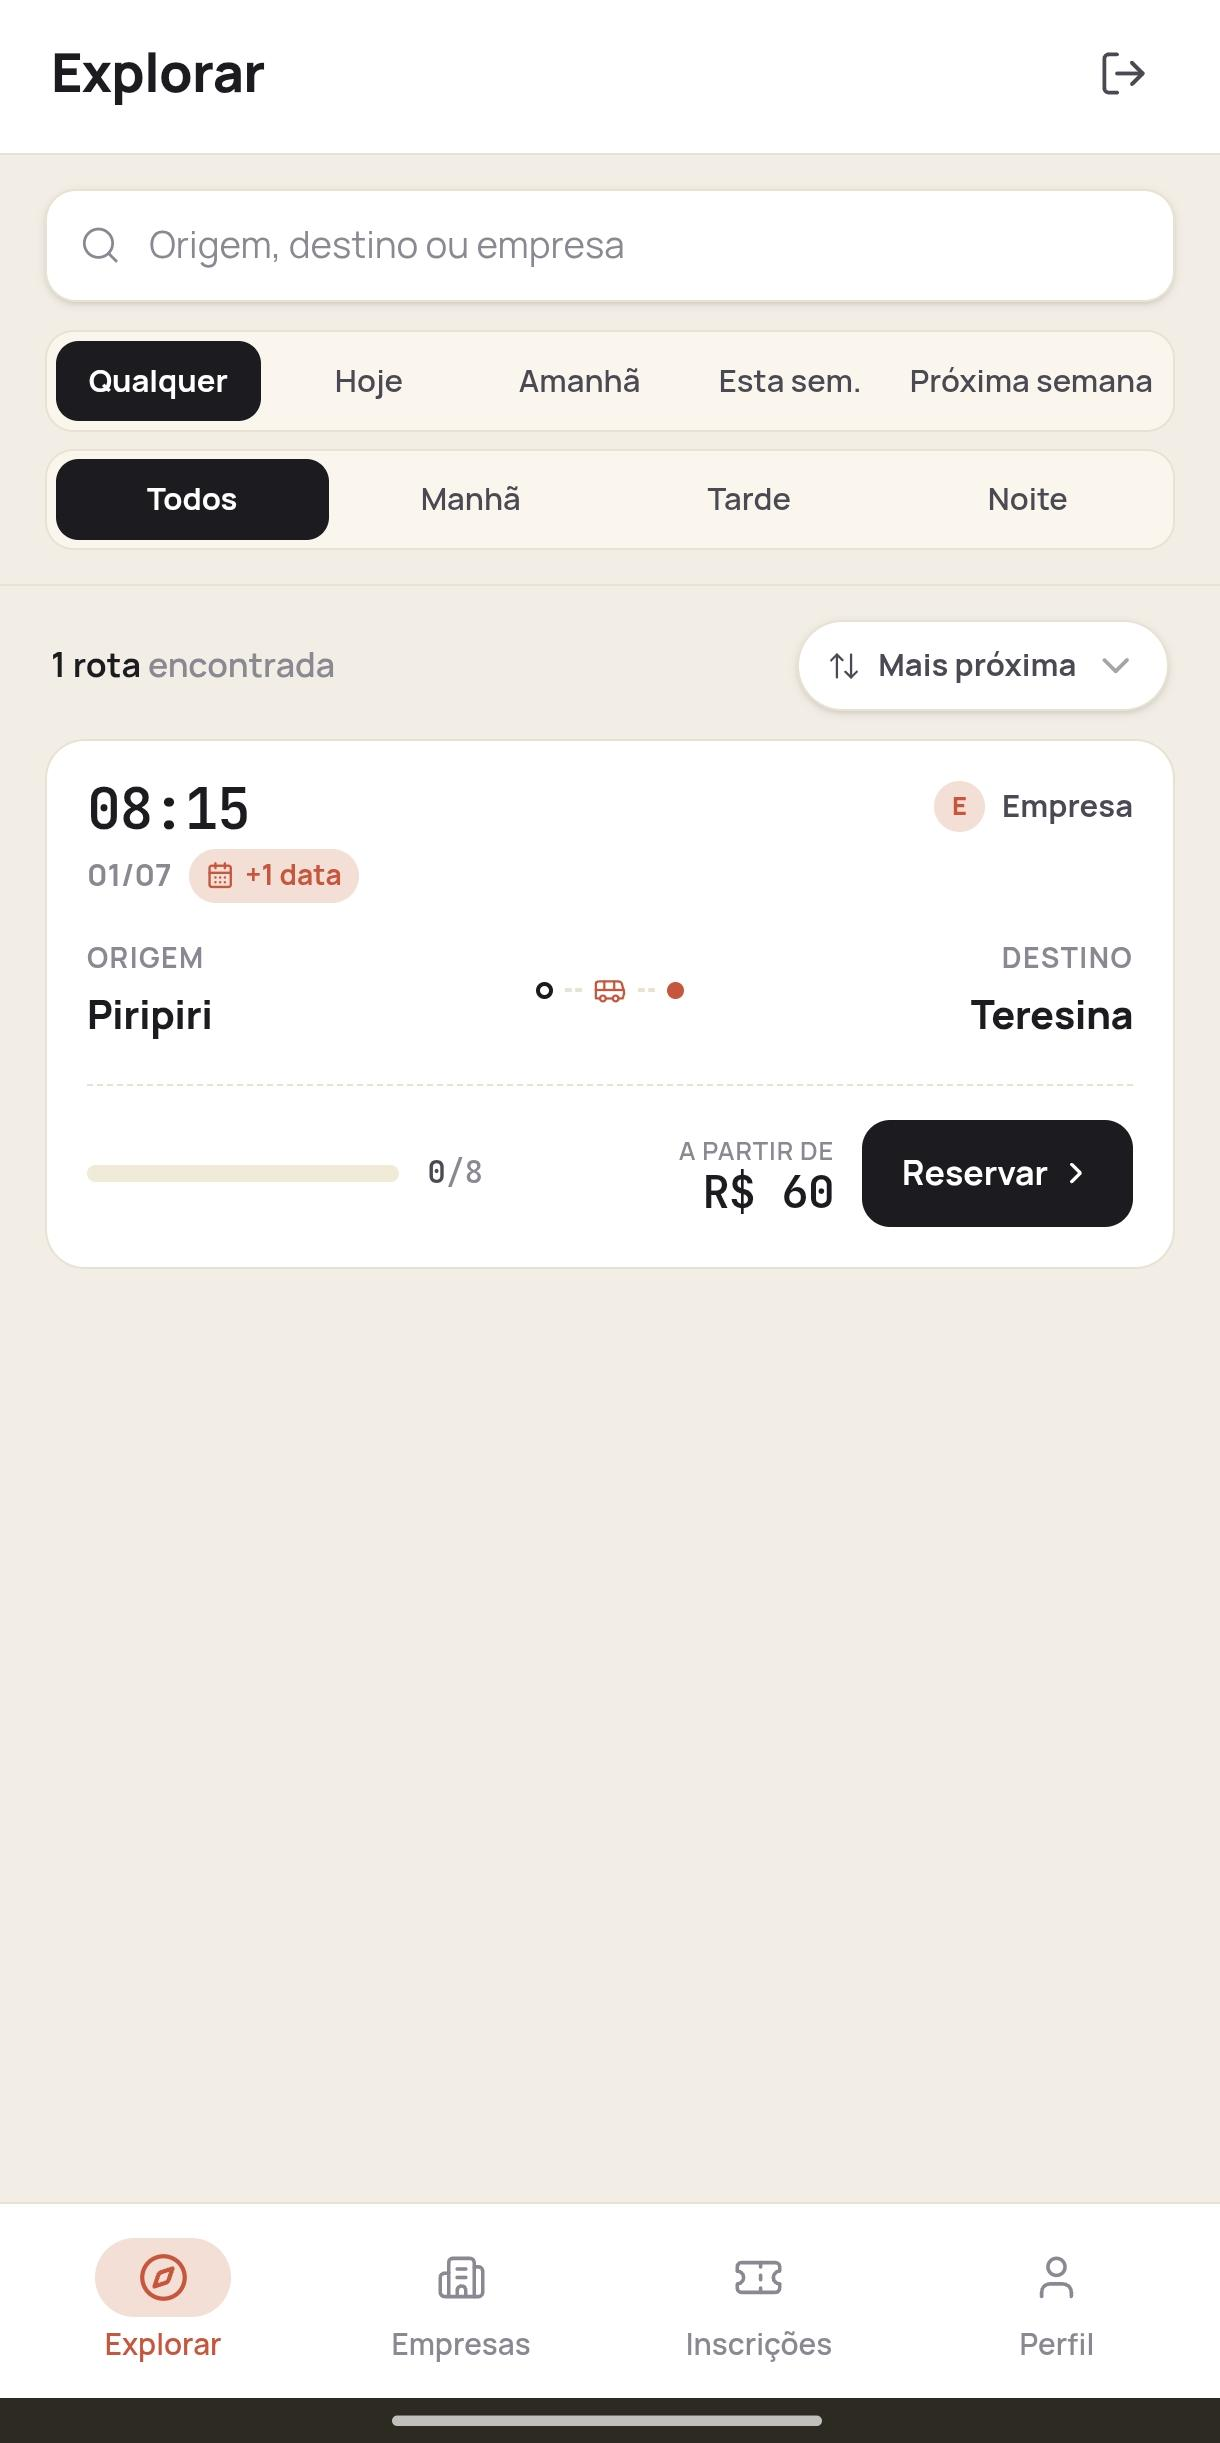
\includegraphics[width=0.5\textwidth]{imagens/fe-catalogo.png}
% \caption{Catálogo público de viagens (marketplace).}
% \label{fig:fe-catalogo}
% \end{figure}
%
% Sugestão de capturas: (1) catálogo público; (2) detalhe da viagem;
% (3) formulário de inscrição; (4) painel administrativo (dashboard);
% (5) tela de detalhe da viagem com gestão de inscrições (presença/pagamento).

\textit{[As capturas de tela das principais interfaces devem ser inseridas neste ponto, conforme as figuras sugeridas no código-fonte.]}

% ------------------------------
\section{Implementação e Resultados Alcançados}

O desenvolvimento contemplou os treze módulos funcionais previstos para o sistema, todos seguindo rigorosamente os padrões de \textit{Clean Architecture} e estruturados com casos de uso, \textit{value objects}, repositórios e tratamento de erros específicos de domínio. Esta seção descreve primeiro a implementação do \textit{backend} (módulos e \textit{endpoints}), em seguida a da aplicação cliente que o consome e, por fim, os temas transversais ao sistema --- autenticação e RBAC, multi-tenancy, transações, tratamento de erros e verificação.

\subsection{Módulos da API (13 Módulos)}

A API expõe 93 endpoints REST distribuídos pelos módulos de domínio, totalizando 93 casos de uso. A Tabela~\ref{tab:endpoints} consolida a contagem por módulo; nas subseções seguintes, cada módulo é descrito com seus casos de uso e endpoints representativos (a especificação completa das rotas está disponível via Swagger em \texttt{/api}).

O \textit{backend} também contou com assistência de IA generativa, porém com um papel mais restrito e de natureza distinta da observada na aplicação cliente. Empregou-se o \textbf{GitHub Copilot} como ferramenta de apoio --- para \textbf{refinar ideias, automatizar trechos repetitivos de código} (como a estrutura recorrente de casos de uso, \textit{value objects} e \textit{mappers}) e \textbf{auxiliar na tomada de decisões} de implementação. A modelagem de domínio, a definição da arquitetura, as regras de negócio e os padrões adotados permaneceram, contudo, sob autoria e revisão do autor. Diferentemente do cliente --- gerado inicialmente por IA e posteriormente refatorado ---, o \textit{backend} foi concebido e escrito de forma incremental pelo autor, cabendo à IA um papel de assistência pontual e de aumento de produtividade.

\begin{table}[H]
\centering
\caption{Endpoints REST e casos de uso por módulo}
\label{tab:endpoints}
\begin{tabular}{lrr}
\toprule
\textbf{Módulo} & \textbf{Endpoints} & \textbf{Use Cases} \\
\midrule
Auth & 9 & 10 \\
User & 8 & 6 \\
Organization & 9 & 8 \\
Membership & 8 & 8 \\
Driver & 9 & 9 \\
Vehicle & 5 & 5 \\
Trip & 17 & 19 \\
Bookings & 10 & 10 \\
Plans & 6 & 6 \\
Subscriptions & 5 & 5 \\
Payment & 4 & 4 \\
Scheduling & 2 & 2 \\
Plan-Usage & 1 & 1 \\
\midrule
\textbf{Total} & \textbf{93} & \textbf{93} \\
\bottomrule
\end{tabular}
\end{table}

\subsubsection{Role Management}

\textbf{Descrição}: Sistema de papéis (roles) que define permissões de acesso (Status: Implementado).

\textbf{Funcionalidades}:
\begin{itemize}
\item Entidade Role com enum de dois papéis: ADMIN e DRIVER.
\item Repositório de Roles com persistência e recuperação.
\item Seed automático que popula roles no banco no primeiro boot.
\item Integração com Docker Compose para inicialização automática.
\end{itemize}

\textbf{Endpoints}: N/A (Roles são pré-definidas no sistema)

\subsubsection{Shared Module}

\textbf{Descrição}: Módulo centralizado que expõe componentes reutilizáveis em todos os contextos delimitados (Status: Implementado).

\textbf{Componentes Exportados}:
\begin{itemize}
\item PrismaModule: Conexão e injeção com o banco de dados.
\item JwtGuard: Guard global para autenticação JWT.
\item RolesGuard, TenantFilterGuard, DevGuard: Guards de autorização.
\item LoggingInterceptor: Interceptador de logging centrado.
\item AllExceptionsFilter: Filter global de tratamento de exceções.
\item Value Objects: Email, Telephone, Money (com validações).
\item UnitOfWork + DbContext: Transações atômicas via AsyncLocalStorage.
\item Domain Errors: Classes base para erros de negócio.
\end{itemize}

\subsubsection{User Module (CRUD + Autenticação)}

\textbf{Descrição}: Gerenciamento completo de usuários e autenticação via JWT (Status: Implementado).

\textbf{Use Cases Implementados}:
\begin{enumerate}
\item CreateUserUseCase: Cadastro com validação de email único e hash de senha Bcrypt.
\item FindAllUsersUseCase: Listagem paginada de usuários ativos.
\item FindUserByIdUseCase: Busca individual com validação 404.
\item UpdateUserUseCase: Atualização com re-validação de dados.
\item DeleteUserUseCase: Soft-delete alterando status para INACTIVE.
\item LoginUseCase: Autenticação com geração de JWT + refresh token.
\item RegisterUseCase: Auto-registro de novo usuário.
\item RefreshTokenUseCase: Renovação de token expirado.
\item RegisterOrganizationWithAdminUseCase: Fluxo unificado de onboarding — cria usuário, organização e membership ADMIN atomicamente via \texttt{UnitOfWork}, com rollback automático pelo Prisma em caso de falha.
\item SetupOrganizationForExistingUserUseCase: Cria organização para usuário já autenticado, gera membership ADMIN e re-emite JWT com o novo \texttt{organizationId} no payload.
\end{enumerate}

\textbf{Endpoints}: 9 rotas de autenticação --- \texttt{POST /auth/\{login, register, refresh, logout, register-organization, setup-organization, forgot-password, reset-password, verify-email\}} --- e o CRUD de usuários (\texttt{POST/GET/PUT/DELETE /users}, com \texttt{GET} paginado e \textit{soft-delete} no \texttt{DELETE}).

\textbf{Segurança}: Bcrypt (salt rounds: 10) para hash de senhas; JWT com secrets distintos para access (1h) e refresh tokens (7d). O payload do JWT é enriquecido no login com todos os dados necessários, eliminando consultas ao banco em cada requisição. O módulo implementa ainda \textbf{recuperação de senha} e \textbf{verificação de e-mail} por tokens de uso único armazenados apenas como hash SHA-256 (TTL de 1h e 24h), com resposta constante na solicitação (anti-enumeration) e revogação de \textit{refresh tokens} via \texttt{jti} no \textit{logout} e na redefinição de senha.

\subsubsection{Organization Module (CRUD)}

\textbf{Descrição}: Gerenciamento de organizações de transporte com multi-tenancy (Status: Implementado).

\textbf{Use Cases Implementados}:
\begin{enumerate}
\item CreateOrganizationUseCase: Criação com slug auto-gerado e validação CNPJ.
\item FindAllOrganizationsUseCase: Listagem paginada de todas (ativas e inativas).
\item FindAllActiveOrganizationsUseCase: Apenas organizações com status ACTIVE.
\item FindOrganizationByIdUseCase: Busca individual com erro 404 e \texttt{OrganizationForbiddenError} (HTTP 403).
\item UpdateOrganizationUseCase: Atualização com re-validação.
\item DisableOrganizationUseCase: Soft-delete com timestamp.
\item FindOrganizationByUserUseCase: Retorna orgs associadas ao \texttt{userId} do token JWT.
\end{enumerate}

\textbf{Endpoints}: 9 rotas. Exemplos: \texttt{GET /organizations/me} (orgs do usuário autenticado), \texttt{GET /organizations/active} (apenas ativas, paginado), \texttt{PUT/DELETE /organizations/:id} (atualização e \textit{soft-delete}). Há ainda endpoints públicos sem autenticação --- \texttt{GET /public/organizations} (lista paginada) e \texttt{GET /public/organizations/:slug} --- para páginas institucionais.

\textbf{Value Objects}: CNPJ (com dígitos verificadores), OrganizationName, Slug (URL-safe), Address.

\subsubsection{Membership Module}

\textbf{Descrição}: Associações entre usuários, roles e organizações. Base fundamental para RBAC (Status: Implementado).

\textbf{Estrutura}: Tabela de junção \textit{OrganizationMembership} com chave composta (userId, roleId, organizationId).

\textbf{Use Cases Implementados}:
\begin{enumerate}
\item CreateMembershipUseCase: O \texttt{organizationId} vem exclusivamente do JWT, eliminando o vetor de ataque cross-tenant. Valida pré-requisito de perfil Driver antes de criar membership com role DRIVER.
\item FindMembershipByCompositeKeyUseCase: Busca específica.
\item FindMembershipsByUserUseCase: Listagem paginada filtrada pela org do caller.
\item FindMembershipsByOrganizationUseCase: Listagem paginada por organização.
\item RemoveMembershipUseCase: Soft-delete via \texttt{removedAt} timestamp.
\item RestoreMembershipUseCase: Reversão de soft-delete.
\item FindRoleByUserIdAndOrganizationIdUseCase: Retorna o role do usuário em uma organização.
\end{enumerate}

\textbf{Endpoints}: 8 rotas operando sobre a chave composta. Exemplos: \texttt{POST /memberships} (org vem do JWT), \texttt{GET /memberships/me/role/:organizationId}, \texttt{DELETE} (\textit{soft-delete}) e \texttt{PATCH .../restore} sobre \texttt{/:userId/:roleId/:organizationId}.

\textbf{Erros de Domínio}: \texttt{MembershipAlreadyExistsError} (HTTP 409), \texttt{MembershipNotFoundError} (HTTP 404), \texttt{DriverNotFoundForMembershipError} (HTTP 400).

\subsubsection{Driver Module}

\textbf{Descrição}: Gerenciamento de perfis de motoristas com Value Objects para CNH. Motoristas são entidades globais — o vínculo com organizações ocorre exclusivamente via \texttt{OrganizationMembership}, permitindo que um usuário seja motorista em múltiplas organizações (Status: Implementado).

\textbf{Fluxo de Onboarding de Motorista}:
\begin{enumerate}
\item Usuário cria perfil via \texttt{POST /drivers} (self-service; \texttt{userId} do JWT).
\item Admin verifica identidade via \texttt{GET /drivers/lookup?email=\&cnh=}.
\item Admin vincula à organização via \texttt{POST /memberships} com \texttt{roleId=DRIVER}.
\end{enumerate}

\textbf{Use Cases Implementados (9 total)}:
\begin{enumerate}
\item CreateDriverUseCase: Criação self-service com check de duplicata (\texttt{DriverAlreadyExistsError} HTTP 409).
\item UpdateDriverUseCase: Atualização (fluxo admin) com verificação de ownership.
\item UpdateOwnDriverUseCase: Atualização parcial self-service (\texttt{cnhExpiresAt}/\texttt{cnhCategories}) via \texttt{PATCH /drivers/me}.
\item FindDriverByIdUseCase: Busca com proteção IDOR via \texttt{belongsToOrganization}.
\item FindDriverByUserIdUseCase: Busca por usuário.
\item FindDriverNameByIdUseCase: Retorna o nome do motorista (visível a passageiros).
\item FindAllDriversByOrganizationUseCase: Paginação com JOIN via membership.
\item RemoveDriverUseCase: Soft delete com validação de ownership.
\item LookupDriverUseCase: Verificação cruzada email + CNH para administrador.
\end{enumerate}

\textbf{Value Objects}: \textbf{Cnh} (9--12 caracteres alfanuméricos) e \textbf{CnhCategories} --- coleção de categorias (A--E) com deduplicação, ordenação e normalização \textit{case-insensitive}, permitindo que um motorista possua múltiplas categorias (ex.: A+B).

\textbf{Endpoints}: 9 rotas. Exemplos: \texttt{POST /drivers} (perfil \textit{self-service}), \texttt{GET /drivers/me}, \texttt{PATCH /drivers/me} (atualização parcial de \texttt{cnhExpiresAt}/\texttt{cnhCategories}), \texttt{GET /drivers/lookup?email=\&cnh=} (ADMIN), \texttt{GET /drivers/organization/:orgId} (paginado) e \texttt{GET /drivers/:id/name} (visível a qualquer usuário autenticado).

\subsubsection{Vehicle Module}

\textbf{Descrição}: Gerenciamento de frota de veículos com Value Object para placa e proteção IDOR (Status: Implementado).

\textbf{Use Cases Implementados (5 total)}:
\begin{enumerate}
\item CreateVehicleUseCase: Criação com validação de placa única (\texttt{PlateAlreadyInUseError} HTTP 409).
\item FindVehicleByIdUseCase: Busca com proteção IDOR via \texttt{organizationId} do JWT.
\item FindAllVehiclesByOrganizationUseCase: Listagem paginada por organização.
\item UpdateVehicleUseCase: Atualização com proteção IDOR e verificação de status ativo (\texttt{VehicleInactiveError} HTTP 410).
\item RemoveVehicleUseCase: Soft-delete com proteção IDOR.
\end{enumerate}

\textbf{Value Objects}: \textbf{Plate} — valida placa brasileira nos formatos \texttt{ABC1234} (padrão) e \texttt{ABC1D23} (Mercosul).

\textbf{Endpoints}: 5 rotas. Exemplos: \texttt{POST/GET /vehicles/organization/:organizationId} (registro e listagem paginada) e \texttt{GET/PUT/DELETE /vehicles/:id} (consulta, atualização e \textit{soft-delete}, todas com proteção IDOR).

\subsubsection{Trip Module}

\textbf{Descrição}: Módulo de viagens com separação entre templates (configuração recorrente) e instâncias (execuções reais), máquina de estados e atribuição de motorista/veículo (Status: Implementado).

\textbf{TripTemplate --- Use Cases (5 total)}:
\begin{enumerate}
\item CreateTripTemplateUseCase: Cria template com configuração de preços por tipo de trajeto.
\item FindTripTemplateByIdUseCase: Busca com proteção IDOR.
\item FindAllTripTemplatesByOrganizationUseCase: Listagem paginada por organização.
\item UpdateTripTemplateUseCase: Atualização com validações de acesso e status.
\item DeactivateTripTemplateUseCase: Soft-deactivation via \texttt{status = INACTIVE}.
\end{enumerate}

\textbf{TripInstance --- Use Cases (7 total)}:
\begin{enumerate}
\item CreateTripInstanceUseCase: Criação a partir de template com propagação de campos.
\item FindTripInstanceByIdUseCase: Busca individual com proteção IDOR.
\item FindAllTripInstancesByOrganizationUseCase: Listagem paginada por organização.
\item FindTripInstancesByTemplateUseCase: Listagem paginada por template.
\item TransitionTripInstanceStatusUseCase: Máquina de estados da viagem.
\item AssignDriverToTripInstanceUseCase: Atribuição/desatribuição de motorista com validação de existência.
\item AssignVehicleToTripInstanceUseCase: Atribuição/desatribuição de veículo com validação de existência.
\end{enumerate}

\textbf{Endpoints}: 17 rotas. \textit{TripTemplate}: CRUD em \texttt{/trip-templates} mais \texttt{POST /trip-templates/:id/generate-instances} (geração manual). \textit{TripInstance}: \texttt{POST /trip-instances}, listagens por org/template, \texttt{GET /trip-instances/driver/me} (viagens do motorista), \texttt{PATCH /trip-instances/:id/status} (máquina de estados) e \texttt{:id/driver}, \texttt{:id/vehicle} (atribuição). Há ainda rotas públicas \texttt{GET /public/trip-instances} e \texttt{.../org/:slug}.

\textbf{Máquina de Estados}:

\begin{table}[H]
\centering
\caption{Transições de status de TripInstance}
\label{tab:trip_status}
\begin{tabular}{lccccc}
\toprule
\textbf{De $\backslash$ Para} & \textbf{SCHEDULED} & \textbf{CONFIRMED} & \textbf{IN\_PROGRESS} & \textbf{FINISHED} & \textbf{CANCELED} \\
\midrule
DRAFT & \checkmark* & -- & -- & -- & \checkmark \\
SCHEDULED & -- & \checkmark* & -- & -- & \checkmark \\
CONFIRMED & \checkmark & -- & \checkmark* & -- & \checkmark \\
IN\_PROGRESS & -- & -- & -- & \checkmark & \checkmark \\
FINISHED & -- & -- & -- & -- & -- \\
CANCELED & -- & -- & -- & -- & -- \\
\bottomrule
\end{tabular}
\end{table}
{\footnotesize * Exige driver e vehicle atribuídos. Transições inválidas lançam \texttt{InvalidTripStatusTransitionError} (HTTP 422).}

\subsubsection{Bookings Module}

\textbf{Descrição}: Gerenciamento completo de inscrições de passageiros em viagens, com controle de capacidade, preço registrado server-side e proteção contra race conditions (Status: Implementado).

\textbf{Use Cases Implementados (9 total)}:
\begin{enumerate}
\item CreateBookingUseCase: Inscreve passageiro com validação de status da viagem, controle de capacidade e preço calculado server-side a partir do template. Todo o fluxo é executado atomicamente via \texttt{UnitOfWork} com isolamento \texttt{Serializable}, prevenindo race conditions clássicas de sistemas de reservas.
\item CancelBookingUseCase: Cancela inscrição com bloqueio para viagens \texttt{IN\_PROGRESS}/\texttt{FINISHED} e prazo de 30 minutos antes da partida.
\item ConfirmPresenceUseCase: Confirma presença do passageiro (apenas org members; owner bloqueado).
\item FindBookingByIdUseCase: Busca com isolamento de tenant.
\item FindBookingsByOrganizationUseCase: Listagem paginada por organização.
\item FindBookingsByTripInstanceUseCase: Lista passageiros de uma viagem (apenas org members).
\item FindBookingsByUserUseCase: Bookings do próprio usuário com filtro de status opcional.
\item FindBookingDetailsUseCase: Detalhe enriquecido com dados da \texttt{TripInstance} (horário, capacidade, vagas disponíveis).
\item GetBookingAvailabilityUseCase: Verifica disponibilidade de vagas antes da inscrição.
\end{enumerate}

\textbf{Endpoints}: 10 rotas. Exemplos: \texttt{POST /bookings} (preço \textit{server-side}), \texttt{GET /bookings/availability/:tripInstanceId} (vagas), \texttt{GET /bookings/:id/details} (detalhe enriquecido), \texttt{PATCH /bookings/:id/cancel} e \texttt{.../confirm-presence} (confirmação restrita a \textit{org members}).

\textbf{Erros de Domínio}: \texttt{BookingNotFoundError} (404), \texttt{BookingAlreadyExistsError} (409), \texttt{TripInstanceFullError} (409), \texttt{TripInstanceNotBookableError} (400), \texttt{BookingCancellationNotAllowedError} (400), \texttt{BookingCancellationDeadlineError} (400), \texttt{BookingAlreadyInactiveError} (400), \texttt{BookingAccessForbiddenError} (403), entre outros.

\subsubsection{Plans Module}

\textbf{Descrição}: Gerenciamento dos planos de assinatura disponíveis na plataforma. Escritas restritas a desenvolvedores via \texttt{DevGuard} (Status: Implementado).

\textbf{Use Cases (5 total)}: \texttt{CreatePlanUseCase}, \texttt{UpdatePlanUseCase}, \texttt{DeactivatePlanUseCase}, \texttt{FindPlanByIdUseCase}, \texttt{FindAllPlansUseCase}.

\textbf{Endpoints}: 6 rotas. Escritas restritas a \texttt{@Dev()} (\texttt{POST /plans}, \texttt{PATCH /plans/:id}, \texttt{.../deactivate}); leitura autenticada (\texttt{GET /plans}, \texttt{/plans/:id}) e endpoint público \texttt{GET /public/plans} para a tela de \textit{onboarding}.

\subsubsection{Subscriptions Module}

\textbf{Descrição}: Gerenciamento de assinaturas das organizações nos planos. Implementa expiração lazy (sem cron job) e controle de limites de plano via \texttt{PlanLimitService} (Status: Implementado).

\textbf{Expiração Lazy}: O helper \texttt{resolveActiveSubscription(orgId, repo)} centraliza a busca + verificação de expiração. Se a assinatura estiver vencida, é transicionada para \texttt{PAST\_DUE} on-demand no momento da leitura.

\textbf{PlanLimitService}: Centraliza verificação de limites de plano (veículos, motoristas, viagens/mês). Injetável em qualquer use case que precise bloquear criação de recursos além da cota.

\textbf{Use Cases (4 total)}:
\begin{enumerate}
\item SubscribeToPlanUseCase: Valida plano ativo e ausência de assinatura ACTIVE. Calcula \texttt{expiresAt = startDate + plan.durationDays}.
\item CancelSubscriptionUseCase: Transita para CANCELED.
\item FindActiveSubscriptionUseCase: Retorna assinatura ativa com lazy expiry.
\item FindSubscriptionsByOrganizationUseCase: Histórico paginado.
\end{enumerate}

\textbf{Endpoints}: 5 rotas sob \texttt{/organizations/:orgId/subscriptions}. Exemplos: \texttt{POST} (assinar plano), \texttt{PATCH /:id/cancel}, \texttt{GET /active} (assinatura vigente, com \textit{lazy expiry}) e \texttt{GET} (histórico paginado).

\subsubsection{Payment Module}

\textbf{Descrição}: Registro e simulação de pagamentos associados a inscrições. A criação de pagamentos é responsabilidade do \texttt{CreateBookingUseCase} — cada inscrição gera automaticamente um registro de pagamento com status \texttt{PENDING}. Os endpoints de simulação permitem demonstrar o fluxo completo sem gateway externo (Status: Implementado). Além do ADMIN, o motorista pode confirmar/falhar pagamentos de viagens atribuídas a ele (\texttt{PaymentNotAssignedToDriverError}, HTTP 403). A resposta inclui \texttt{tripInstanceId} e \texttt{tripDepartureTime} (\textit{snapshots} de leitura), permitindo ao cliente agregar receita por data da viagem.

\textbf{Use Cases (4 total)}: \texttt{FindPaymentByIdUseCase}, \texttt{FindPaymentsByOrganizationUseCase}, \texttt{ConfirmPaymentUseCase} (\texttt{PENDING → COMPLETED}), \texttt{FailPaymentUseCase} (\texttt{PENDING → FAILED}).

\textbf{Endpoints}: 4 rotas sob \texttt{/organizations/:orgId/payments}. \texttt{GET /:id} e \texttt{GET} (listagem paginada); \texttt{PATCH /:id/confirm} (\texttt{PENDING → COMPLETED}) e \texttt{.../fail} (\texttt{PENDING → FAILED}), simulando o ciclo sem gateway externo.

\subsubsection{Scheduling Module}

\textbf{Descrição}: Automação da geração e do encerramento de viagens recorrentes via \textit{jobs} agendados (\texttt{@nestjs/schedule}), parametrizados por organização através de \texttt{TripSchedulingConfig} (Status: Implementado).

\textbf{Jobs (\textit{cron})}:
\begin{enumerate}
\item \textbf{Geração recorrente} (\texttt{0 2 * * *} UTC): para cada organização ativa, materializa uma janela rolante de \texttt{TripInstance} a partir dos \texttt{TripTemplate} recorrentes, respeitando \texttt{daysAhead} e a cota de viagens do plano. Idempotente por (template, dia).
\item \textbf{Auto-cancelamento} (\texttt{*/15 * * * *} UTC): transiciona para \texttt{CANCELED} as instâncias cujo prazo (\texttt{autoCancelAt}) venceu sem atingir a receita mínima, propagando a falha aos pagamentos \texttt{PENDING} associados.
\end{enumerate}

\textbf{Use Cases (3 total)}: \texttt{FindTripSchedulingConfigUseCase}, \texttt{UpdateTripSchedulingConfigUseCase} e a geração manual \texttt{GenerateTripInstancesForTemplateUseCase} (mesmo núcleo do \textit{cron}, exposta via \texttt{POST /trip-templates/:id/generate-instances}).

\textbf{Endpoints}: 2 rotas sob \texttt{/organizations/:organizationId/scheduling-config} (\texttt{GET} e \texttt{PATCH}, ADMIN). A cadência dos \textit{jobs} é fixa; a configuração por organização controla apenas a janela (\texttt{daysAhead}) e a ativação (\texttt{enabled}). O \texttt{ScheduleModule} é registrado condicionalmente (\texttt{DISABLE\_CRON}).

\subsubsection{Plan-Usage Module}

\textbf{Descrição}: Exposição consolidada do consumo de recursos da organização frente aos limites do plano vigente, para alimentar painéis administrativos (Status: Implementado).

\textbf{Use Case (1 total)}: \texttt{FindPlanUsageUseCase} --- agrega contagem de veículos, motoristas e viagens (estas contadas dentro do \textbf{período de assinatura} corrente, \texttt{[startDate, expiresAt)}, e não por mês-calendário) e confronta com \texttt{maxVehicles}, \texttt{maxDrivers} e \texttt{maxMonthlyTrips}.

\textbf{Endpoints}: 1 rota --- \texttt{GET /organizations/:id/plan-usage}.

\subsection{Aplicação Cliente}
\label{sec:cliente}

A aplicação cliente é um \textit{Single Page Application} (SPA) \textit{mobile-first} que consome os 93 \textit{endpoints} da API e materializa, para os perfis de passageiro, motorista e administrador, os fluxos descritos na Seção~\ref{sec:interfaces}.

\subsubsection{Processo de Desenvolvimento Assistido por IA}

A aplicação cliente foi \textbf{integralmente desenvolvida com o apoio de ferramentas de inteligência artificial (IA) generativa}, sob direção, revisão e validação do autor. Esse modelo de trabalho --- frequentemente denominado \textit{AI-assisted development} ou programação assistida por IA --- foi adotado de forma deliberada para acelerar a prototipação e a implementação, mantendo-se a autoria das decisões de requisitos, de arquitetura e de qualidade sob responsabilidade humana. Registra-se o uso dessas ferramentas em conformidade com as boas práticas de transparência acadêmica. O processo organizou-se em três etapas sequenciais e complementares, cada uma apoiada por uma ferramenta distinta.

Na primeira etapa, de \textbf{geração inicial}, a base do projeto foi produzida com a plataforma \textbf{Lovable}, ferramenta de geração de aplicações assistida por IA, que estabeleceu o esqueleto da aplicação --- a \textit{stack} React com TanStack Router, Tailwind CSS e shadcn/ui --- e um primeiro conjunto de telas funcionais. Na segunda etapa, de \textbf{concepção visual}, o \textbf{Claude Design} (da Anthropic) foi empregado para \textbf{aprimorar as telas existentes e gerar novos protótipos de alta fidelidade}, apoiando as decisões de \textit{layout}, de hierarquia visual e de sistema de design. Na terceira etapa, de \textbf{implementação real}, o assistente de programação agêntico \textbf{Claude Code} (também da Anthropic) foi utilizado para escrever, refatorar e evoluir o código de produção e para \textbf{realizar a integração efetiva com o \textit{backend}}, sempre a partir de instruções do autor e com revisão do resultado. É importante destacar que \textbf{as telas geradas nas etapas iniciais foram posteriormente refatoradas e aprimoradas} na fase de implementação: o código foi reorganizado na arquitetura de \textit{feature modules}, as chamadas à API foram centralizadas na camada de serviços, o controle de acesso por papel foi consolidado nos \textit{layouts} de rota e a apresentação foi unificada sob um sistema de design coeso. Dessa forma, a IA atuou como ferramenta de produtividade ao longo de todo o ciclo --- da prototipação à integração ---, enquanto a estrutura, os padrões e a qualidade final do código resultam das decisões e da revisão conduzidas pelo autor.

\subsubsection{Roteamento e Controle de Acesso}

O roteamento utiliza o mecanismo \textit{file-based} do TanStack Router, no qual a estrutura de nomes dos arquivos determina a árvore de URLs. \textit{Layouts} sem caminho (prefixados por sublinhado) não acrescentam segmento à URL, mas estabelecem nós sob os quais outras rotas são aninhadas, permitindo associar a um conjunto de rotas uma verificação de acesso comum. A autenticação é verificada uma única vez, no \textit{layout} \texttt{\_protected}, que envolve todas as rotas que exigem sessão; sobre essa base, dois \textit{layouts} adicionais --- \texttt{\_admin} e \texttt{\_driver} --- aplicam as verificações de papel, redirecionando usuários sem o papel correspondente. A composição resulta em uma cadeia de verificações (autenticado \textbf{e} administrador, por exemplo), sem que os segmentos de proteção apareçam na URL. Esse modelo é o reflexo, no cliente, do RBAC implementado pelos \textit{guards} do \textit{backend}.

\subsubsection{Padrão de Serviços e Hooks}

O Código~\ref{cod:fe_camadas} ilustra o fluxo unidirecional através das camadas: um serviço expõe operações de alto nível sobre os \textit{endpoints}; um \textit{hook} de caso de uso combina o serviço com estado e lógica de apresentação (busca, filtros), derivando o estado de carregamento da ausência simultânea de conteúdo e erro; e uma rota fina apenas decide entre os estados (carregando, erro, conteúdo) e delega a renderização.

\begin{lstlisting}[language=JavaScript, caption={Fluxo entre as camadas: serviço, hook e rota}, label={cod:fe_camadas}]
// SERVICO (services/bookings.service.ts) - padrao repositorio
export const bookingsService = {
  listForUser: () => api("/bookings/user"),
  cancel: (id) => api(`/bookings/${id}/cancel`, { method: "PATCH" }),
};

// HOOK (features/bookings/hooks/useBookings.ts) - caso de uso
export function useBookings() {
  const [bookings, setBookings] = useState(null);
  const [error, setError] = useState(null);
  useEffect(() => {
    bookingsService.listForUser()
      .then((res) => setBookings(res.data ?? res))
      .catch((err) => { setError(err.message); toast.error(err.message); });
  }, []);
  return { bookings, loading: bookings === null && !error, error };
}

// ROTA (routes/_protected.my-bookings.tsx) - controlador fino
function MyBookingsContent() {
  const { bookings, loading, error } = useBookings();
  return (
    <AppShell title="Minhas inscricoes">
      {loading ? <LoadingList /> :
       error ? <ErrorCard message={error} /> :
       <BookingsList bookings={bookings} />}
    </AppShell>
  );
}
\end{lstlisting}

\subsubsection{Integração com a API}

A comunicação com o \textit{backend} é concentrada no cliente HTTP (Código~\ref{cod:fe_api}) e organizada pela camada de serviços. Os aspectos mais relevantes dessa integração são:

\textbf{Autenticação.} Toda requisição é autenticada por padrão, com o cabeçalho \texttt{Authorization: Bearer}; chamadas a \textit{endpoints} públicos desabilitam esse comportamento explicitamente. A expiração do \textit{access token} é tratada de forma transparente pela renovação automática descrita na Seção~\ref{sec:autenticacao}.

\textbf{Endpoints públicos.} As telas do contexto público consomem rotas anônimas expostas pela API --- \texttt{GET /public/trip-instances}, \texttt{GET /public/organizations} (e \texttt{/:slug}) e \texttt{GET /public/plans} ---, permitindo a descoberta de viagens, organizações e planos sem autenticação, em conformidade com o funil de conversão do produto.

\textbf{Contexto multi-tenant.} O isolamento por organização é responsabilidade do \textit{backend} (campo \texttt{organizationId} e \texttt{TenantFilterGuard}); no cliente, o contexto de papel deriva a organização administrada do usuário cruzando \texttt{GET /organizations/me} com \texttt{GET /memberships/me/role/:organizationId}, padrão também reutilizado para listar as organizações em que o usuário atua como motorista.

\textbf{Apresentação temporal.} A API armazena horários recorrentes em UTC; o cliente os converte e exibe sempre em horário de Brasília, e nunca expõe \textit{cron expressions} ou horários UTC literais ao usuário.

\subsection{Autenticação e Autorização (RBAC)}
\label{sec:autenticacao}

A segurança de acesso é definida no \textit{backend} e refletida no cliente. No servidor, o fluxo de autenticação JWT compreende: (i) \textbf{registro}, com a senha \textit{hasheada} com Bcrypt (10 \textit{salt rounds}) antes da persistência; (ii) \textbf{login}, que valida credenciais e emite um \textit{access token} de curta duração (1 hora) e um \textit{refresh token} de longa duração (7 dias); (iii) \textbf{refresh}, em que o cliente troca o \textit{refresh token} por um novo par; e (iv) \textbf{proteção de rotas}, na qual o \texttt{JwtAuthGuard} valida o \textit{access token} e responde 401 quando inválido ou expirado.

O pipeline de segurança é composto por quatro \textit{guards} executados em sequência (Código~\ref{cod:auth_pipeline}):

\begin{lstlisting}[caption={Pipeline de autorização do backend}, label={cod:auth_pipeline}]
Request
  -> JwtAuthGuard      # valida JWT; constroi TenantContext -> req.context
  -> RolesGuard        # verifica @Roles(); isDev ignora
  -> TenantFilterGuard # :organizationId param == req.context.organizationId
  -> DevGuard          # apenas isDev=true passa em rotas @Dev()
  -> Controller
\end{lstlisting}

O \texttt{JwtAuthGuard} enriquece o \textit{payload} JWT no momento do login com todos os dados necessários (\texttt{userId}, \texttt{organizationId}, \texttt{role}, \texttt{isDev}), eliminando consultas ao banco a cada requisição. Usuários listados em \texttt{DEV\_EMAILS} recebem \texttt{isDev=true} no token e ignoram validações de tenant e role. Em termos de papéis, o \textbf{ADMIN} tem acesso total (organizações, usuários, motoristas, configurações), o \textbf{DRIVER} tem acesso limitado (visualizar viagens e confirmar ações relacionadas) e o \textbf{USER} implícito (passageiro) pode inscrever-se em viagens e visualizar suas inscrições. As \textit{memberships} permitem múltiplas \textit{roles} por usuário em diferentes organizações (ex.: motorista em uma org, admin em outra).

\textbf{Reflexo no cliente.} A aplicação persiste a sessão em \texttt{localStorage} (\textit{token} de acesso, \textit{token} de renovação e dados básicos do usuário) e provê o estado de autenticação por meio de dois contextos encadeados: um de autenticação, que envolve um de papel, garantindo que a determinação de papel só ocorra quando a identidade já está disponível. A principal característica de resiliência é a \textbf{renovação transparente de sessão}: diante de uma resposta \texttt{401}, o cliente dispara uma única renovação --- \textbf{deduplicada} entre requisições concorrentes --- e repete a chamada original, conforme o Código~\ref{cod:fe_api}.

\begin{lstlisting}[language=JavaScript, caption={Cliente HTTP com renovação transparente de sessão (\texttt{lib/api.ts})}, label={cod:fe_api}]
export async function api(path, init = {}) {
  const { auth = true, _retry = false, headers, ...rest } = init;
  if (auth && tokenStorage.access)
    headers.Authorization = `Bearer ${tokenStorage.access}`;

  const res = await fetch(`${API_BASE_URL}${path}`, { ...rest, headers });

  // Tenta uma unica renovacao (deduplicada) em caso de 401 e repete a chamada.
  if (res.status === 401 && auth && !_retry) {
    if (!refreshPromise)
      refreshPromise = doRefresh().finally(() => { refreshPromise = null; });
    try { await refreshPromise; return api(path, { ...init, _retry: true }); }
    catch { /* renovacao falhou - propaga o erro original */ }
  }
  if (!res.ok) throw new ApiError(message, res.status, data, errorCode);
  return data;
}
\end{lstlisting}

\subsection{Multi-tenancy}

O isolamento lógico de dados entre organizações é implementado no \textit{backend} através de:
\begin{enumerate}
\item \textbf{Campo organizationId}: Presente em todas as entidades que pertencem a uma organização.
\item \textbf{Filtragem em Queries}: Todas as buscas filtram por \texttt{organizationId} da organização do usuário autenticado.
\item \textbf{TenantFilterGuard}: Valida que o parâmetro \texttt{:organizationId} na rota corresponde ao \texttt{organizationId} do JWT.
\item \textbf{Proteção IDOR (OWASP A01)}: Endpoints com parâmetro \texttt{/:id} validam ownership via \texttt{organizationId} do JWT em Driver, Vehicle e Trip.
\end{enumerate}

\subsection{Infraestrutura Transacional --- UnitOfWork + DbContext}

Para garantir atomicidade em operações que envolvem múltiplas escritas (ex: criar \texttt{Booking} + \texttt{Payment}), foi implementada uma infraestrutura de transações baseada em \texttt{AsyncLocalStorage}:

\begin{lstlisting}[caption={Fluxo de transação via UnitOfWork}, label={cod:uow}]
UseCase
  -> unitOfWork.execute(async () => {
       await bookingRepository.save(booking)
       await paymentRepository.save(payment)
     })
         |
PrismaUnitOfWork
  -> prisma.$transaction((tx) =>
       dbContext.run(tx, fn))   # coloca tx no AsyncLocalStorage
           |
DbContext (AsyncLocalStorage)
  -> client = tx durante a execucao
           |
Repository -> usa dbContext.client automaticamente
\end{lstlisting}

Fora de transação, \texttt{dbContext.client} aponta para o \texttt{PrismaService} (cliente raiz). Dentro da transação, aponta para o \texttt{tx}. A camada de aplicação não conhece Prisma e não precisa alterar assinaturas de repositórios.

\subsection{Tratamento de Erros Estruturado}

O sistema implementa hierarquia de exceções mapeadas pelo \texttt{AllExceptionsFilter} global do \textit{backend}, conforme a Tabela~\ref{tab:error_mapping}.

\begin{table}[H]
\centering
\caption{Mapeamento de erros de domínio para HTTP}
\label{tab:error_mapping}
\begin{tabular}{ll}
\toprule
\textbf{Sufixo do código de erro} & \textbf{HTTP} \\
\midrule
\texttt{\_NOT\_FOUND} & 404 Not Found \\
\texttt{\_ALREADY\_EXISTS} & 409 Conflict \\
\texttt{INVALID\_} / \texttt{\_BAD\_REQUEST} & 400 Bad Request \\
\texttt{\_FORBIDDEN} & 403 Forbidden \\
\texttt{\_UNAUTHORIZED} & 401 Unauthorized \\
\texttt{\_GONE} & 410 Gone \\
\bottomrule
\end{tabular}
\end{table}

\textbf{Reflexo no cliente.} A interface decide a mensagem a apresentar a partir do \textbf{código de erro de domínio} fornecido pela API (campo \texttt{error} do \textit{payload}), e não do texto da mensagem. O cliente normaliza toda falha em uma exceção tipada (\texttt{ApiError}) que carrega \texttt{status}, dados e o \texttt{errorCode}; um módulo central traduz esses códigos --- alinhados ao mapeamento da Tabela~\ref{tab:error_mapping} --- para mensagens em português, distinguindo, por exemplo, limites de plano excedidos (com ação que conduz à tela de assinatura), prazos de cancelamento de inscrição e \textit{tokens} de redefinição expirados.

\subsection{Banco de Dados: Migrações e Seed}

Prisma gerencia histórico completo de mudanças no esquema com migrations versionadas. O script \texttt{prisma/seed.ts} popula automaticamente roles padrão (ADMIN, DRIVER), planos (FREE, BASIC, PRO, PREMIUM) e um usuário admin de teste.

\subsection{Verificação}

\subsubsection{Testes Unitários do Backend}

\textbf{Status Atual}: 458 testes em 57 suites, cobrindo os use cases críticos de todos os módulos, guards de autorização e fluxos de negócio complexos.

\textbf{Padrão de Testes Adotado}:
\begin{itemize}
\item \textbf{AAA (Arrange-Act-Assert)}: Estrutura consistente em todas as suites.
\item \textbf{makeMocks()}: Cria todos os mocks via \texttt{jest.fn()} com tipagem \texttt{jest.Mocked<T>}.
\item \textbf{setupHappyPath()}: Configura mocks para o cenário de sucesso padrão.
\item \textbf{Injeção manual}: Dependências injetadas diretamente, sem mocks de framework NestJS.
\item \textbf{Factories}: Funções \texttt{make*()} por módulo com suporte a overrides parciais.
\end{itemize}

A Tabela~\ref{tab:testes} resume a cobertura agregada por módulo; o detalhamento por use case está versionado no repositório (\texttt{test/modules/}).

\begin{table}[H]
\centering
\caption{Cobertura de testes unitários agregada por módulo}
\label{tab:testes}
\begin{tabular}{lrr}
\toprule
\textbf{Módulo} & \textbf{Suites} & \textbf{Testes} \\
\midrule
Trip & 18 & 183 \\
Bookings & 9 & 88 \\
Auth & 7 & 36 \\
Driver & 4 & 33 \\
Shared (Guards) & 3 & 26 \\
Payment & 3 & 20 \\
Subscriptions & 3 & 18 \\
Scheduling & 2 & 15 \\
Membership & 1 & 10 \\
Organization & 2 & 10 \\
Vehicle & 2 & 7 \\
User & 2 & 6 \\
Plans & 1 & 6 \\
\midrule
\textbf{Total} & \textbf{57} & \textbf{458} \\
\bottomrule
\end{tabular}
\end{table}

Os testes apoiam-se em \textit{factories} por módulo (funções \texttt{make*()} com suporte a \textit{overrides} parciais) que constroem entidades de domínio e DTOs de entrada --- por exemplo \texttt{makeUser}, \texttt{makeOrganization}, \texttt{makeDriver}, \texttt{makeTripTemplate}, \texttt{makeTripInstance}, \texttt{makeBooking}, \texttt{makeSubscription} ---, eliminando duplicação de \textit{setup} entre as suites.

\subsubsection{Verificação do Frontend}

Em coerência com o estágio do produto e o tamanho reduzido da equipe, a estratégia de verificação do frontend é, no momento, \textbf{predominantemente manual}, estruturada em um roteiro de dezenas de cenários que cobrem os caminhos principais, os fluxos que cruzam contextos de acesso e os casos de borda. A integração contínua executa a verificação de estilo, a análise estática e a construção, deixando a verificação funcional a cargo do roteiro manual. A adoção de testes automatizados (provavelmente Vitest com \textit{Testing Library} para \textit{hooks} e serviços, e uma ferramenta de ponta a ponta para os fluxos) está condicionada à aproximação da operação comercial, tendo o fluxo de reserva como primeiro candidato à cobertura. A Tabela~\ref{tab:testes_manuais} ilustra o formato dos casos de teste manuais.

\begin{table}[H]
\centering
\caption{Exemplos de casos de teste manuais do frontend}
\label{tab:testes_manuais}
\begin{tabular}{lll}
\toprule
\textbf{Caso} & \textbf{Resultado esperado} & \textbf{Status} \\
\midrule
Login com credenciais válidas & Sessão criada e redirecionamento por papel & OK \\
Login com credenciais inválidas & Mensagem de erro, sem sessão & OK \\
Expiração do \textit{token} durante navegação & Renovação transparente, ação concluída & OK \\
Mesmo ponto de embarque e desembarque & Bloqueio com mensagem de validação & OK \\
Cancelamento fora da janela permitida & Bloqueio com mensagem do \textit{errorCode} & OK \\
Rota administrativa sem papel de admin & Redirecionamento para a raiz & OK \\
\bottomrule
\end{tabular}
\end{table}

% ------------------------------
\section{Considerações Finais}
\label{sec:consideracoes}

\subsection{Síntese dos Resultados}

O projeto alcançou os objetivos estabelecidos, com a implementação completa dos treze módulos funcionais planejados (93 \textit{endpoints} REST e 93 casos de uso) e da aplicação cliente que os consome. O sistema demonstra uma arquitetura sólida baseada em \textit{Clean Architecture} e \textit{Domain-Driven Design} no servidor, espelhada por uma arquitetura em camadas no cliente. Entre os resultados de maior relevância de engenharia, destacam-se:

\begin{enumerate}
\item \textbf{Arquitetura Modular Espelhada}: Cada módulo do servidor segue o padrão Application → Domain → Infrastructure → Presentation; o cliente reproduz a separação em rotas finas, \textit{hooks} de caso de uso, serviços e cliente HTTP único, conferindo localidade de mudança e previsibilidade a ambos os lados.
\item \textbf{Multi-tenancy}: Isolamento lógico de dados via \texttt{organizationId} em todas as entidades pertinentes, com \texttt{TenantFilterGuard} e proteção IDOR (OWASP A01) nos \textit{endpoints} por ID.
\item \textbf{Autenticação e RBAC}: JWT com \textit{access tokens} de curta duração e \textit{refresh tokens}, Bcrypt (10 \textit{salt rounds}), \textit{guards} de autorização e suporte a múltiplas \textit{roles} por usuário; no cliente, controle de acesso por papel centralizado nos \textit{layouts} e renovação de sessão transparente.
\item \textbf{Value Objects e Soft-delete}: Encapsulamento de validações críticas (CNPJ, Email, Slug, CNH, Placa, Money) e preservação de histórico via exclusão lógica nas entidades críticas.
\item \textbf{Viagens e Automação}: TripTemplate + TripInstance com máquina de estados, atribuição de motorista/veículo e \textit{jobs} de geração recorrente e auto-cancelamento por organização.
\item \textbf{Inscrições e Transações Atômicas}: Bookings com controle de capacidade, preço calculado \textit{server-side} e proteção contra \textit{race conditions} via \texttt{UnitOfWork} com isolamento \texttt{Serializable}.
\item \textbf{Planos, Assinaturas e Pagamentos}: Modelo SaaS com \textit{tiers}, limites de recursos (\texttt{PlanLimitService}), expiração \textit{lazy} e simulação do ciclo de pagamento (PENDING → COMPLETED/FAILED).
\item \textbf{Tratamento de Erros e CI/CD}: \texttt{AllExceptionsFilter} global com mapeamento estável de códigos de erro, consumido pelo cliente; \textit{rate limiting} global (60 req/min); \textit{pipeline} de \textit{build}, \textit{lint} e testes via GitHub Actions.
\item \textbf{Verificação}: 458 testes unitários em 57 \textit{suites} no \textit{backend} (padrão AAA, \textit{factories} por módulo) e roteiro de testes manuais no cliente.
\end{enumerate}

\subsubsection{Métricas do Projeto}

\begin{table}[H]
\centering
\caption{Métricas de progresso do sistema Movy}
\label{tab:metricas_projeto}
\begin{tabular}{lrr}
\toprule
\textbf{Métrica} & \textbf{Total} & \textbf{Implementado} \\
\midrule
Módulos funcionais & 13 & 13 \\
Use Cases & 93 & 93 \\
Endpoints REST & 93 & 93 \\
Entidades de Domínio & 14 & 14 \\
Migrações Executadas & 28 & 28 \\
Testes unitários (backend) & --- & 458 testes / 57 suites \\
CI/CD (GitHub Actions) & Configurado & \checkmark \\
Rate Limiting & Configurado & 60 req/min \\
\bottomrule
\end{tabular}
\end{table}

\subsection{Limitações Identificadas}

O sistema cobre o escopo de módulos planejado, mas mantém limitações conscientes, documentadas aqui como decisões datadas e revisáveis, e não como omissões.

\begin{enumerate}
\item \textbf{Integração com Gateway de Pagamento}: O módulo de pagamentos opera com simulação de ciclo de vida (PENDING → COMPLETED/FAILED). A integração com um gateway real (ex.: Stripe) é a próxima evolução natural do módulo.
\item \textbf{Notificações}: O sistema de notificações por e-mail/SMS ainda não foi implementado, afetando os requisitos RF17 e RF18.
\item \textbf{Relatórios}: As funcionalidades de geração de relatórios e históricos (RF15, RF16) ainda não foram desenvolvidas no \textit{backend}; o cliente já dispõe de relatório financeiro agregado no painel administrativo.
\item \textbf{Cobertura de Testes}: Embora 458 testes cubram os use cases críticos e os \textit{guards} principais, alguns use cases secundários ainda não possuem \textit{specs} dedicadas, e o cliente carece de testes automatizados (verificação atualmente manual).
\item \textbf{Caching}: Não há \textit{caching} (ex.: Redis) para otimização de consultas frequentes.
\item \textbf{Frontend --- decisões conscientes}: suporte, no estágio atual, a uma única organização por administrador (a primeira retornada por \texttt{GET /organizations/me}); coexistência de dois estilos de obtenção de dados pela não adoção imediata de uma biblioteca de estado de servidor; e armazenamento de credenciais em \texttt{localStorage}, aceito em troca de simplicidade e marcado para reavaliação antes da operação comercial.
\end{enumerate}

\subsection{Lições Aprendidas}

\begin{enumerate}
\item \textbf{Clean Architecture é Essencial}: A separação clara entre camadas facilitou desenvolvimento iterativo e testes de componentes isolados, tanto no servidor quanto, por espelhamento, no cliente.
\item \textbf{DDD Agregou Valor}: Value Objects bem definidos preveniram bugs de validação e documentam regras de negócio naturalmente.
\item \textbf{Multi-tenancy Desde o Início}: Implementar multi-tenancy na arquitetura inicial foi crítico; retroajustar seria custoso.
\item \textbf{Segurança IDOR Requer Vigilância Ativa}: Endpoints com parâmetro \texttt{/:id} sem \texttt{:organizationId} na rota exigem validação explícita de ownership via \texttt{organizationId} do JWT ou método \texttt{belongsToOrganization()} no repositório.
\item \textbf{Desacoplamento de Módulos Previne Ciclos}: O padrão Orchestrator (Auth coordenando User, Organization, Membership) eliminou dependências circulares e violações do SRP.
\item \textbf{Testes AAA com Injeção Manual são Superiores}: Dependências injetadas manualmente tornam os testes mais rápidos e isolados, e forçam o código a ser testável por design.
\item \textbf{Um Único Ponto de Comunicação com a API}: Concentrar no cliente HTTP a autenticação, a renovação de sessão e a normalização de erros permitiu tratar questões transversais de forma uniforme em todo o cliente.
\end{enumerate}

\subsection{Recomendações para Continuação}

\subsubsection{Ações Imediatas Recomendadas}

\begin{enumerate}
\item \textbf{Integração de Pagamentos}: Configurar gateway real (Stripe) para substituir a simulação atual, conectando-o ao fluxo de inscrições.
\item \textbf{Notificações}: Implementar notificações via e-mail/SMS (RF17, RF18) utilizando Bull/BullMQ para processamento assíncrono.
\item \textbf{Expandir Cobertura de Testes}: Adicionar \textit{specs} para use cases secundários do \textit{backend} e introduzir uma camada de testes automatizados no cliente, a partir do fluxo de reserva.
\item \textbf{Fortalecer a Sessão no Cliente}: Reavaliar o armazenamento de credenciais em \texttt{localStorage} antes da operação comercial.
\item \textbf{Backup Strategy}: Configurar backups automáticos do banco PostgreSQL em desenvolvimento e produção.
\end{enumerate}

\subsubsection{Tecnologias Futuras a Considerar}

\begin{itemize}
\item \textbf{Redis}: Para caching de dados frequentes e gerenciamento de sessões.
\item \textbf{Bull/BullMQ}: Para fila de jobs assíncronos (notificações, relatórios).
\item \textbf{TanStack Query}: Para unificar o gerenciamento de estado de servidor no cliente.
\item \textbf{Sentry/Rollbar}: Para monitoramento de erros em produção.
\item \textbf{DataDog/New Relic}: Para APM (Application Performance Monitoring).
\end{itemize}

\subsection{Conclusão}

O sistema Movy demonstra viabilidade técnica e arquitetural para operar como uma plataforma SaaS de gerenciamento de transporte universitário intermunicipal. Os princípios de \textit{Clean Architecture} e DDD forneceram, no servidor, uma fundação sólida que antecipa o crescimento futuro sem sacrificar manutenibilidade; e a aplicação cliente, ao espelhar essa estratificação e ao concentrar a comunicação com a API em um ponto único, materializa os requisitos do sistema com controle de acesso por papel e comunicação resiliente.

Com os treze módulos funcionais implementados --- autenticação, usuários, organizações, papéis, \textit{memberships}, motoristas, veículos, viagens, inscrições, planos, assinaturas, pagamentos e agendamento ---, um sistema robusto de RBAC, multi-tenancy e proteção IDOR, e 458 testes unitários no \textit{backend}, o projeto entrega uma plataforma funcional ponta a ponta. As limitações registradas --- gateway de pagamento, notificações, relatórios, \textit{caching} e a maturação da camada de testes do cliente --- delineiam um roteiro de evolução claro, cujos pontos de inserção já estão previstos na arquitetura atual.

% ------------------------------
\newpage
\renewcommand{\refname}{}
\section*{Referências}
\bibliographystyle{abntex2-num}
\bibliography{referencias}

% ------------------------------
\newpage
\section*{Anexos}

\subsection*{Declaração de Entrega do Código-Fonte}
Declaro que o código-fonte foi entregue à coordenação do curso xxxxx

Assinatura: \rule{10cm}{0.4pt}

Data: \rule{1cm}{0.4pt}/\rule{1cm}{0.4pt}/\rule{2cm}{0.4pt}

\subsection*{Declaração de Submissão ao NIT}
Declaro que o software foi submetido ao NIT – IFPI xxxxx

Assinatura: \rule{10cm}{0.4pt}

Data: \rule{1cm}{0.4pt}/\rule{1cm}{0.4pt}/\rule{2cm}{0.4pt}

\end{document}
